% Options for packages loaded elsewhere
\PassOptionsToPackage{unicode}{hyperref}
\PassOptionsToPackage{hyphens}{url}
%
\documentclass[
]{book}
\usepackage{amsmath,amssymb}
\usepackage{lmodern}
\usepackage{iftex}
\ifPDFTeX
  \usepackage[T1]{fontenc}
  \usepackage[utf8]{inputenc}
  \usepackage{textcomp} % provide euro and other symbols
\else % if luatex or xetex
  \usepackage{unicode-math}
  \defaultfontfeatures{Scale=MatchLowercase}
  \defaultfontfeatures[\rmfamily]{Ligatures=TeX,Scale=1}
\fi
% Use upquote if available, for straight quotes in verbatim environments
\IfFileExists{upquote.sty}{\usepackage{upquote}}{}
\IfFileExists{microtype.sty}{% use microtype if available
  \usepackage[]{microtype}
  \UseMicrotypeSet[protrusion]{basicmath} % disable protrusion for tt fonts
}{}
\makeatletter
\@ifundefined{KOMAClassName}{% if non-KOMA class
  \IfFileExists{parskip.sty}{%
    \usepackage{parskip}
  }{% else
    \setlength{\parindent}{0pt}
    \setlength{\parskip}{6pt plus 2pt minus 1pt}}
}{% if KOMA class
  \KOMAoptions{parskip=half}}
\makeatother
\usepackage{xcolor}
\usepackage{color}
\usepackage{fancyvrb}
\newcommand{\VerbBar}{|}
\newcommand{\VERB}{\Verb[commandchars=\\\{\}]}
\DefineVerbatimEnvironment{Highlighting}{Verbatim}{commandchars=\\\{\}}
% Add ',fontsize=\small' for more characters per line
\usepackage{framed}
\definecolor{shadecolor}{RGB}{248,248,248}
\newenvironment{Shaded}{\begin{snugshade}}{\end{snugshade}}
\newcommand{\AlertTok}[1]{\textcolor[rgb]{0.94,0.16,0.16}{#1}}
\newcommand{\AnnotationTok}[1]{\textcolor[rgb]{0.56,0.35,0.01}{\textbf{\textit{#1}}}}
\newcommand{\AttributeTok}[1]{\textcolor[rgb]{0.77,0.63,0.00}{#1}}
\newcommand{\BaseNTok}[1]{\textcolor[rgb]{0.00,0.00,0.81}{#1}}
\newcommand{\BuiltInTok}[1]{#1}
\newcommand{\CharTok}[1]{\textcolor[rgb]{0.31,0.60,0.02}{#1}}
\newcommand{\CommentTok}[1]{\textcolor[rgb]{0.56,0.35,0.01}{\textit{#1}}}
\newcommand{\CommentVarTok}[1]{\textcolor[rgb]{0.56,0.35,0.01}{\textbf{\textit{#1}}}}
\newcommand{\ConstantTok}[1]{\textcolor[rgb]{0.00,0.00,0.00}{#1}}
\newcommand{\ControlFlowTok}[1]{\textcolor[rgb]{0.13,0.29,0.53}{\textbf{#1}}}
\newcommand{\DataTypeTok}[1]{\textcolor[rgb]{0.13,0.29,0.53}{#1}}
\newcommand{\DecValTok}[1]{\textcolor[rgb]{0.00,0.00,0.81}{#1}}
\newcommand{\DocumentationTok}[1]{\textcolor[rgb]{0.56,0.35,0.01}{\textbf{\textit{#1}}}}
\newcommand{\ErrorTok}[1]{\textcolor[rgb]{0.64,0.00,0.00}{\textbf{#1}}}
\newcommand{\ExtensionTok}[1]{#1}
\newcommand{\FloatTok}[1]{\textcolor[rgb]{0.00,0.00,0.81}{#1}}
\newcommand{\FunctionTok}[1]{\textcolor[rgb]{0.00,0.00,0.00}{#1}}
\newcommand{\ImportTok}[1]{#1}
\newcommand{\InformationTok}[1]{\textcolor[rgb]{0.56,0.35,0.01}{\textbf{\textit{#1}}}}
\newcommand{\KeywordTok}[1]{\textcolor[rgb]{0.13,0.29,0.53}{\textbf{#1}}}
\newcommand{\NormalTok}[1]{#1}
\newcommand{\OperatorTok}[1]{\textcolor[rgb]{0.81,0.36,0.00}{\textbf{#1}}}
\newcommand{\OtherTok}[1]{\textcolor[rgb]{0.56,0.35,0.01}{#1}}
\newcommand{\PreprocessorTok}[1]{\textcolor[rgb]{0.56,0.35,0.01}{\textit{#1}}}
\newcommand{\RegionMarkerTok}[1]{#1}
\newcommand{\SpecialCharTok}[1]{\textcolor[rgb]{0.00,0.00,0.00}{#1}}
\newcommand{\SpecialStringTok}[1]{\textcolor[rgb]{0.31,0.60,0.02}{#1}}
\newcommand{\StringTok}[1]{\textcolor[rgb]{0.31,0.60,0.02}{#1}}
\newcommand{\VariableTok}[1]{\textcolor[rgb]{0.00,0.00,0.00}{#1}}
\newcommand{\VerbatimStringTok}[1]{\textcolor[rgb]{0.31,0.60,0.02}{#1}}
\newcommand{\WarningTok}[1]{\textcolor[rgb]{0.56,0.35,0.01}{\textbf{\textit{#1}}}}
\usepackage{longtable,booktabs,array}
\usepackage{calc} % for calculating minipage widths
% Correct order of tables after \paragraph or \subparagraph
\usepackage{etoolbox}
\makeatletter
\patchcmd\longtable{\par}{\if@noskipsec\mbox{}\fi\par}{}{}
\makeatother
% Allow footnotes in longtable head/foot
\IfFileExists{footnotehyper.sty}{\usepackage{footnotehyper}}{\usepackage{footnote}}
\makesavenoteenv{longtable}
\usepackage{graphicx}
\makeatletter
\def\maxwidth{\ifdim\Gin@nat@width>\linewidth\linewidth\else\Gin@nat@width\fi}
\def\maxheight{\ifdim\Gin@nat@height>\textheight\textheight\else\Gin@nat@height\fi}
\makeatother
% Scale images if necessary, so that they will not overflow the page
% margins by default, and it is still possible to overwrite the defaults
% using explicit options in \includegraphics[width, height, ...]{}
\setkeys{Gin}{width=\maxwidth,height=\maxheight,keepaspectratio}
% Set default figure placement to htbp
\makeatletter
\def\fps@figure{htbp}
\makeatother
\setlength{\emergencystretch}{3em} % prevent overfull lines
\providecommand{\tightlist}{%
  \setlength{\itemsep}{0pt}\setlength{\parskip}{0pt}}
\setcounter{secnumdepth}{5}
\ifLuaTeX
\usepackage[bidi=basic]{babel}
\else
\usepackage[bidi=default]{babel}
\fi
\babelprovide[main,import]{brazilian}
% get rid of language-specific shorthands (see #6817):
\let\LanguageShortHands\languageshorthands
\def\languageshorthands#1{}
\usepackage{booktabs}
\ifLuaTeX
  \usepackage{selnolig}  % disable illegal ligatures
\fi
\usepackage[]{natbib}
\bibliographystyle{plainnat}
\IfFileExists{bookmark.sty}{\usepackage{bookmark}}{\usepackage{hyperref}}
\IfFileExists{xurl.sty}{\usepackage{xurl}}{} % add URL line breaks if available
\urlstyle{same} % disable monospaced font for URLs
\hypersetup{
  pdftitle={Bookdown Meus Resumos},
  pdfauthor={Daniel Claudino},
  pdflang={pt-BR},
  hidelinks,
  pdfcreator={LaTeX via pandoc}}

\title{Bookdown Meus Resumos}
\author{Daniel Claudino}
\date{2022-11-01}

\begin{document}
\maketitle

{
\setcounter{tocdepth}{1}
\tableofcontents
}
\hypertarget{apresentauxe7uxe3o}{%
\chapter{Apresentação}\label{apresentauxe7uxe3o}}

Bookdown Meus Resumos

\begin{figure}

{\centering 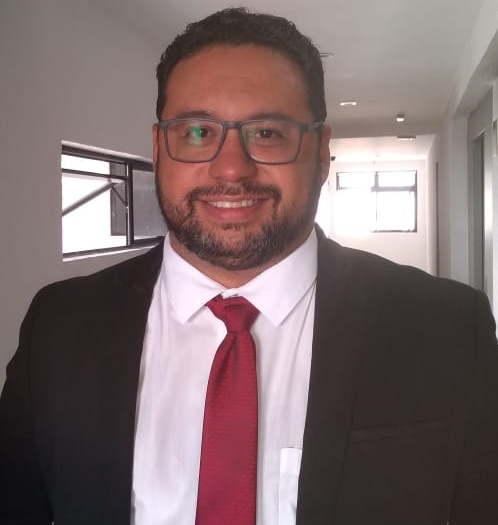
\includegraphics[width=0.5\linewidth]{imagens/FOTO-PERFIL-DANIEL-CLAUDINO-2020} 

}

\caption{Autor: Daniel Claudino}\label{fig:unnamed-chunk-1}
\end{figure}

Neste bookdown estarão contidos os resumos de:
* Capítulos de livros
* Artigos
* Monografias
* Dissertações
* Teses
* Notícias de jornais

Esses materiais estarão relacionados com as disciplinas do 1º até o 10º período do curso de Bacharelado em Psicologia, bem como com a elaboração do meu TCC, artigos, dissertações e teses a serem publicados por mim.

\hypertarget{controle-de-versuxe3o}{%
\section{Controle de Versão}\label{controle-de-versuxe3o}}

\begin{longtable}[]{@{}
  >{\raggedright\arraybackslash}p{(\columnwidth - 6\tabcolsep) * \real{0.2500}}
  >{\raggedright\arraybackslash}p{(\columnwidth - 6\tabcolsep) * \real{0.2500}}
  >{\raggedright\arraybackslash}p{(\columnwidth - 6\tabcolsep) * \real{0.2500}}
  >{\raggedright\arraybackslash}p{(\columnwidth - 6\tabcolsep) * \real{0.2500}}@{}}
\toprule()
\begin{minipage}[b]{\linewidth}\raggedright
Versão
\end{minipage} & \begin{minipage}[b]{\linewidth}\raggedright
Data / Hora
\end{minipage} & \begin{minipage}[b]{\linewidth}\raggedright
Colaborador
\end{minipage} & \begin{minipage}[b]{\linewidth}\raggedright
Descrição da Contribuição
\end{minipage} \\
\midrule()
\endhead
0.1 & 01/11/2022 11h34 & \href{https://wa.me/5583988853815}{Daniel Claudino} & Versão inicial do documento \\
\bottomrule()
\end{longtable}

\hypertarget{referuxeancias-bibliogruxe1ficas}{%
\section{Referências Bibliográficas}\label{referuxeancias-bibliogruxe1ficas}}

\hypertarget{bibliografia-buxe1sica}{%
\subsection{Bibliografia Básica}\label{bibliografia-buxe1sica}}

DAVIDOFF, Linda L. Introdução à Psicologia. São Paulo: Makron Books, 2001.

SPINK, M. J. P. Psicologia social e saúde: práticas, saberes e sentidos. Petrópolis:Vozes, 2013.

MAISTO, Albert A.; MORRIS, Charles G. Introdução a Psicologia. 6 ed.~São Paulo, Prentice Hall, 2004. {[}Livro Eletrônico{]}

\hypertarget{bibliografia-complementar}{%
\subsection{Bibliografia Complementar}\label{bibliografia-complementar}}

BRIGAGÃO, J., NASCIMENTO, V. L. V., \& SPINK, P. K. (2011). As interfaces entre psicologia e políticas públicas e a configuração de novos espaços de atuação. Sorocaba, (páginas, 199-215).

CASTRO, E. K., \& BORNHOLDT, E. (2004). Psicologia da saúde x psicologia hospitalar: definições e possibilidades de inserção profissional. Psicologia Ciência e Profissão (páginas, 48-57).

COELHO, Wilson Ferreira. Psicologia do Desenvolvimento. São Paulo: Editora Pearson, 2014. {[}Livro Eletrônico{]}

CÓRIA-SABINI, Maria Aparecida. Psicologia do Desenvolvimento. 2 ed.~São Paulo: Editora Ática, 2010. {[}Livro Eletrônico{]}

DIAS, A. C. G., PATIAS, N. D., \& ABAID, J. L. W. ( 2014). Psicologia escolar e possibilidades na atuação do psicólogo: algumas reflexões. Revista Psicologia Escolar e Educacional (páginas 105-111).

FEIST, J., FEIST, G., \& ROBERTS, T. A. (2015). Teorias da Personalidade.

FELDMAN, Robert S. Introdução à Psicologia. Porto Alegre: Editora AMGH,2015.

ILETTI, Nelson; ROSSATO, Solange Marques; ROSSATO, Geovanio. Psicologia do Desenvolvimento. São Paulo, Contexto, 2014. {[}Livro Eletrônico{]}

LIMA, C. F., \& PIMENTEL, C. E. (2017). Livro: Revisitando a Psicologia Social. MISKOLCI, Richard. Teoria Queer: um aprendizado pelas diferenças. 2 ed.~Belo Horizonte: Autêntica, 2015. {[}Livro Eletrônico{]}

PADILHA, S., NORONHA, A. P. P., \& ZANCHET, C. F. (2007). Instrumentos de avaliação psicológica: uso e parecer de psicólogos. Avaliação psicológica (páginas, 69-79).

SCHULTZ, D. \& SCHULTZ, S. E. (2019). História da Psicologia moderna.

ZANELLI, J. C., BASTOS, A. V. B., \& RODRIGUES, A. C. A. ( 2014). Psicologia, Organizações e Trabalho no Brasil. (Orgs).

\hypertarget{observauxe7uxe3o-importante}{%
\section{Observação Importante}\label{observauxe7uxe3o-importante}}

\textbf{NOTA}: Este material tem como finalidade auxiliar a fixação de assuntos estudados em sala de aula de acordo com o \textbf{plano de ensino desta disciplina}.

Ele \textbf{não deve ser} utilizado como \textbf{único material de estudo para a prova}, então:

\begin{enumerate}
\def\labelenumi{\arabic{enumi}.}
\tightlist
\item
  Consulte os \textbf{slides da professora} na plataforma FTM;\\
\item
  Faça \textbf{notas de aula} do que for tratado em sala de aula;\\
\item
  Consulte nossas \textbf{notas de aula};
\end{enumerate}

\begin{quote}
\textbf{Dúvidas}: Devem ser encaminhadas no grupo de whatsapp da disciplina.
\end{quote}

\hypertarget{p1---anatomia-humana}{%
\chapter{P1 - Anatomia Humana}\label{p1---anatomia-humana}}

Neste capítulo estarão contidos os resumos relacionados com a disciplina Anatomia Humana.

Em breve\ldots{}

\hypertarget{p1---introduuxe7uxe3o-uxe0-psicologia}{%
\chapter{P1 - Introdução à Psicologia}\label{p1---introduuxe7uxe3o-uxe0-psicologia}}

Neste capítulo estarão contidos os resumos relacionados com a disciplina Introdução à Psicologia.

\hypertarget{livro-psicologias-uma-introduuxe7uxe3o-ao-estudo-da-psicologia-boch-furtado-teixeira-2001}{%
\section{\texorpdfstring{Livro: \textbf{Psicologias Uma Introdução ao Estudo da Psicologia} (BOCH; FURTADO; TEIXEIRA, 2001)}{Livro: Psicologias Uma Introdução ao Estudo da Psicologia (BOCH; FURTADO; TEIXEIRA, 2001)}}\label{livro-psicologias-uma-introduuxe7uxe3o-ao-estudo-da-psicologia-boch-furtado-teixeira-2001}}

Figura - Livro Psicologias: Uma Introdução ao Estudo da Psicologia. 13.ed. São Paulo: Saraiva, 2001

capa-livro-psicologias.jpg

\hypertarget{capuxedtulo-3---o-behaviorismo}{%
\subsection{Capítulo 3 - O Behaviorismo}\label{capuxedtulo-3---o-behaviorismo}}

\begin{itemize}
\tightlist
\item
  Em breve, disponibilizaremos.
\end{itemize}

\hypertarget{capuxedtulo-4---a-gestalt}{%
\subsection{Capítulo 4 - A Gestalt}\label{capuxedtulo-4---a-gestalt}}

\hypertarget{a-psicologia-da-forma-introduuxe7uxe3o-uxe0-psicologia-da-gestalt}{%
\subsubsection{A Psicologia da Forma: Introdução à Psicologia da Gestalt}\label{a-psicologia-da-forma-introduuxe7uxe3o-uxe0-psicologia-da-gestalt}}

\begin{itemize}
\tightlist
\item
  Para Bock (2001, p.~59) a Psicologia da Gestalt é uma das tendências teóricas mais \textbf{coerentes} e \textbf{coesas} da história da psicologia.
\item
  O termo Gestalt é de origem alemã e tem significado aproximado ao de \textbf{forma} ou \textbf{configuração}, ****porém**** \textbf{NÃO É UTILIZADO} por não corresponder exatamente as seu real significado em psicologia.
\item
  No final do século XIII, estudiosos procuravam compreender o \textbf{fenômeno psicológico} em seus aspectos naturais.

  \begin{itemize}
  \tightlist
  \item
    Principalmente no sentido da \textbf{mensurabilidade} ( A Psicofísica em voga ).
  \end{itemize}
\end{itemize}

\hypertarget{predecessores-da-psiologia-da-gestalt}{%
\paragraph{Predecessores da Psiologia da Gestalt}\label{predecessores-da-psiologia-da-gestalt}}

\begin{itemize}
\tightlist
\item
  Estudiosos considerados os mais diretos predecessores/antecessores da Psisocologia Gestalt:

  \begin{itemize}
  \tightlist
  \item
    Ernst Mash (1838-1916), físico;
  \item
    Christian von Ehrenfels (1859-1932), fisólofo e psicólogo
  \end{itemize}
\item
  Estudos desenvolvidos:

  \begin{itemize}
  \tightlist
  \item
    Estudos psicofísicos sobre as \textbf{sensações} de \textbf{espaço-forma} e \textbf{tempo-forma}

    \begin{itemize}
    \tightlist
    \item
      Dado Psicológico: Sensações
    \item
      Dados Físico: espaço-forma e tempo-forma
    \end{itemize}
  \end{itemize}
\item
  Fundadores

  \begin{itemize}
  \tightlist
  \item
    Max Wertheimer
  \item
    Wolfgang Kohler
  \item
    Kurt Koffka
  \end{itemize}
\end{itemize}

\hypertarget{fundadores-da-psiologia-da-gestalt}{%
\paragraph{Fundadores da Psiologia da Gestalt}\label{fundadores-da-psiologia-da-gestalt}}

\begin{itemize}
\tightlist
\item
  Os fundadores da Psicologia da Gestalt construíram a \textbf{base de uma teoria psicológica}.
\end{itemize}

\begin{longtable}[]{@{}
  >{\centering\arraybackslash}p{(\columnwidth - 4\tabcolsep) * \real{0.3333}}
  >{\centering\arraybackslash}p{(\columnwidth - 4\tabcolsep) * \real{0.3333}}
  >{\centering\arraybackslash}p{(\columnwidth - 4\tabcolsep) * \real{0.3333}}@{}}
\toprule()
\endhead
Figura - \href{https://translate.google.com/?sl=hu\&tl=pt\&text=Max\%20Wertheimer\&op=translate}{Max Wertheimer :speaker:} (1880-9343) & Figura - \href{https://translate.google.com/?sl=de\&tl=pt\&text=Wolfgang\%20Kohler\&op=translate}{Wolfgang Kohler :speaker:}(1887-1967) & Figura - \href{https://translate.google.com/?sl=de\&tl=pt\&text=Kurt\%20Koffka\&op=translate}{Kurt Koffka :speaker:}(1886-1941) \\
\bottomrule()
\end{longtable}

\textbf{Obs}: Clique em :speaker: para ouvir a pronúncia dos nomes dos cientístas acima.

\begin{itemize}
\tightlist
\item
  Estudos iniciais

  \begin{itemize}
  \tightlist
  \item
    Estudos da percepção e sensação do movimento;
  \item
    Preocupação: Compreender \textbf{quais processos psicológicos} estavam envolvidos na \textbf{ilusão de ótica} quando o estímulo é percebido como uma \textbf{forma} diferente da que o sujeito tem na realidade.

    \begin{itemize}
    \tightlist
    \item
      Exemplo: Cinema; fotogramas estáticos; imagem formada na retina que demora um pouco para ser apagada; ilusão de óptica do movimento (sensação).
    \end{itemize}
  \end{itemize}
\end{itemize}

\hypertarget{a-percepuxe7uxe3o}{%
\subsubsection{A percepção}\label{a-percepuxe7uxe3o}}

\begin{itemize}
\tightlist
\item
  É \textbf{ponto de partida} e \textbf{tema central} da Psicologia da Gestalt;
\item
  Teoria Behaviorista

  \begin{itemize}
  \tightlist
  \item
    \textbf{Princípio Implícito}: Há uma relação de \textbf{causa} e \textbf{efeito} entre o \textbf{estímulo} e a \textbf{resposta}
  \end{itemize}
\item
  Para Gestaltistas há um questionamento desse \textbf{princípio implícito da teoria behaviorista}

  \begin{itemize}
  \tightlist
  \item
    Entre o \textbf{estímulo} e a \textbf{resposta} encontra-se o ****processo de percepção****
  \item
    ****O QUE**** o indivíduo percebe e ****COMO**** o indivíduo percebe ****são importantes para entender o COMPORTAMENTO****
  \end{itemize}
\end{itemize}

\begin{Shaded}
\begin{Highlighting}[]
\NormalTok{flowchart LR}
\NormalTok{OQ(O que){-}{-}A Pessoa Percebe{-}{-}\textgreater{}CC(Entendimento do Comportamento)}
\NormalTok{CM(Como){-}{-}A Pessoa Percebe{-}{-}\textgreater{}CC}
\end{Highlighting}
\end{Shaded}

\hypertarget{posiuxe7uxe3o-de-behavioristas-x-gestaltistas-diante-do-objeto-da-psicologia}{%
\paragraph{Posição de Behavioristas x Gestaltistas diante do Objeto da Psicologia}\label{posiuxe7uxe3o-de-behavioristas-x-gestaltistas-diante-do-objeto-da-psicologia}}

\begin{itemize}
\tightlist
\item
  Ambos definem a psicologia como a ****ciência que estuda o COMPORTAMENTO****
\item
  Para os Behavioristas:

  \begin{itemize}
  \tightlist
  \item
    É mais profunda a preocupação com a \textbf{objetividade};
  \item
    O \textbf{estudo com comportamento} é feito através da \textbf{relação estímulo-resposta};
  \item
    Despreza os ****conteúdos da consciência**** pela impossibilidade de controlar cientificamente \textbf{essas variáveis};
  \item
    Procura isolar o \textbf{estímulo} que corresponderia à \textbf{resposta} desprezando ****conteúdos da consciência**** pela impossibilidade de controlar cientificamente \textbf{essas variáveis};
  \end{itemize}
\item
  Para os gestaltistas:

  \begin{itemize}
  \tightlist
  \item
    Há uma \textbf{crítica} a \textbf{abordagem behaviorista} acima;
  \item
    Acreditam que existe um \textbf{contexto mais amplo} que é importante no \textbf{estudo do comportamento}

    \begin{itemize}
    \tightlist
    \item
      Esse \textbf{contexto mais amplo} são as ****CONDIÇÕES**** que \textbf{afetam/alteram} nossa capacidade de ****PERCEBER**** o \textbf{estímulo};
    \end{itemize}
  \item
    Entendem que estudar o comportamento isolado de um \textbf{contexto mais amplo} pode prejudicar o entendimento do comportamento pelo psicólogo;
  \item
    O comportamento é estudado em seus aspectos mais globais levando em consideração as ****CONDIÇÕES**** que \textbf{afetam/alteram} nossa capacidade de ****PERCEBER**** o \textbf{estímulo}
  \end{itemize}
\end{itemize}

\hypertarget{o-que-garante-o-entendimento-do-que-eu-percebo}{%
\paragraph{O que Garante o Entendimento do que Eu Percebo ?}\label{o-que-garante-o-entendimento-do-que-eu-percebo}}

\begin{itemize}
\tightlist
\item
  Quando eu vejo

  \begin{itemize}
  \tightlist
  \item
    Uma parte de um objeto
  \end{itemize}
\item
  Ocorre uma tendência à

  \begin{itemize}
  \tightlist
  \item
    restauração do \textbf{equilíbrio da forma}
  \end{itemize}
\item
  Garantindo
  * O entendimento do que estou percebendo
\end{itemize}

\hypertarget{o-fenuxf4meno-da-percepuxe7uxe3o}{%
\paragraph{O Fenômeno da Percepção}\label{o-fenuxf4meno-da-percepuxe7uxe3o}}

\begin{itemize}
\tightlist
\item
  É norteado pela busca de

  \begin{itemize}
  \tightlist
  \item
    \textbf{fechamento} dos pontos que compõem uma figura;
  \item
    \textbf{simetria} dos pontos que compõem uma figura;
  \item
    \textbf{regularidade} dos pontos que compõem uma figura;
  \end{itemize}
\item
  \textbf{Rudolf Arnheim} afirma que o \textbf{sentido normal da visão} apreende um \textbf{padrão global};
\end{itemize}

Figura - Lei básica da percepção visual para os psicólogos da Gestalt

\begin{itemize}
\tightlist
\item
  Observações a respeito da Figura:

  \begin{itemize}
  \tightlist
  \item
    \textbf{Figura 1}:

    \begin{itemize}
    \tightlist
    \item
      Percebemos como um \textbf{quadrado} e não como uma \textbf{figura inclinada} ou um \textbf{perfil} (Figura 2)
    \end{itemize}
  \item
    \textbf{Figura 3}:

    \begin{itemize}
    \tightlist
    \item
      Após acrescentarmos quatro pontos, o padrão percebido na Figura 1 irá mudar e perceberemos \textbf{um círculo}
    \end{itemize}
  \item
    \textbf{Figura 4}:

    \begin{itemize}
    \tightlist
    \item
      É possível ver tanto \textbf{círculos brancos} quanto \textbf{quadrados brancos} nos centros das cruzes;
    \end{itemize}
  \end{itemize}
\end{itemize}

\begin{quote}
Qualquer padrão de estímulo tende a ser visto de tal modo que a \textbf{estrutura resultante} é tão \textbf{simples} quanto as \textbf{condições dadas} permitem
\end{quote}

\hypertarget{a-boa-forma}{%
\subsubsection{A boa-forma}\label{a-boa-forma}}

\begin{itemize}
\tightlist
\item
  A Psicologia da Gestalt encontra as \textbf{condições} para a \textbf{compreensão do comportamento humano} nos \textbf{fenômenos da percepção}.
\item
  Em relação aos nossos comportamentos:

  \begin{itemize}
  \tightlist
  \item
    Em alguns casos, \textbf{guardam estreita relação com os estímulos físicos};
  \item
    Em outros casos, \textbf{são completamente diferentes do esperado} porque ``****entendemos o ambiente****'' \textbf{de maneira diferente da sua realidade}.
  \item
    Exemplo:

    \begin{itemize}
    \tightlist
    \item
      Cumprimentar uma pessoas e depois descobrir que cumprimentamos uma pessoa desconhecida (\textbf{Erro de Percepção});
    \end{itemize}
  \end{itemize}
\item
  Não há \textbf{boa forma} quando \textbf{nos elementos percebidos} não há:

  \begin{itemize}
  \tightlist
  \item
    Equilíbrio
  \item
    Simetria
  \item
    Estabilidade
  \item
    Simplicidade
  \end{itemize}
\item
  \textbf{O elemento que objetivamos compreender}

  \begin{itemize}
  \tightlist
  \item
    COMO DEVE SER APRESENTADO

    \begin{itemize}
    \tightlist
    \item
      Deve ser apresentado em \textbf{aspectos básicos} que \textbf{permitam a sua decodificação} (\textbf{percepção da boa forma})
    \end{itemize}
  \end{itemize}
\end{itemize}

Figura - Observe a RETA: Elemento que desejamos compreender

\begin{itemize}
\tightlist
\item
  (\ldots)

  \begin{itemize}
  \tightlist
  \item
    COMO DEVEM SER DISTRIBUÍDOS OS ELEMENTOS QUE O COMPÕEM
    * Para garantir a \textbf{boa forma} devem ser apresentados com
    - Equilíbrio
    - Simetria
    - Estabilidade
    - Simplicidade
  \end{itemize}
\item
  A \textbf{tendência da nossa percepção} em buscar a \textbf{boa forma} permitirá a relação \textbf{figura-fundo}
\item
  Quanto mais clara (simples, estável, simétrica e equilibrada) estiver a \textbf{boa-forma}

  \begin{itemize}
  \tightlist
  \item
    Mais clara será a \textbf{separação} entre \textbf{figura} e \textbf{fundo};
  \end{itemize}
\item
  Quanto menos clara estiver a boa forma

  \begin{itemize}
  \tightlist
  \item
    Mais difícil será distinguir o que é figura e o que é fundo (****Figura Ambígua****);
  \end{itemize}
\end{itemize}

\hypertarget{meio-geogruxe1fico-e-meio-comportamental}{%
\subsubsection{Meio Geográfico e Meio Comportamental}\label{meio-geogruxe1fico-e-meio-comportamental}}

\begin{itemize}
\tightlist
\item
  O comportamento \textbf{É DETERMINADO} pela \textbf{PERCEPÇÃO DO ESTÍMULO};
\item
  O comportamento está/estará sujeito a \textbf{LEI DA BOA-FORMA};
\item
  O \textbf{CONJUNTO DE ESTÍMULOS} determinantes do comportamento é denominado \textbf{MEIO AMBIENTAL} ( ou apenas MEIO )
\item
  Existem DOIS TIPOS DE MEIOS AMBIENTAIS

  \begin{itemize}
  \tightlist
  \item
    \textbf{Meio GEOGRÁFICO}

    \begin{itemize}
    \tightlist
    \item
      É o meio enquanto tal;
    \item
      É o meio físico EM TERMOS OBJETIVOS;
    \end{itemize}
  \item
    \textbf{Meio COMPORTAMENTAL}

    \begin{itemize}
    \tightlist
    \item
      É o meio resultante de INTERAÇÃO (Indivíduo \textless==\textgreater{} Meio Físico)
    \item
      Implica a \textbf{INTERPRETAÇÃO} desse meio através das \textbf{FORÇAS} que regem a \textbf{PERCEPÇÃO};

      \begin{enumerate}
      \def\labelenumi{\alph{enumi}.}
      \tightlist
      \item
        Forças que regem a percepção:
      \item
        Equilíbrio
      \end{enumerate}

      \begin{enumerate}
      \def\labelenumi{\roman{enumi}.}
      \setcounter{enumi}{1}
      \tightlist
      \item
        Simetria
      \item
        Estabilidade
      \item
        Simplicidade
      \end{enumerate}
    \end{itemize}
  \end{itemize}
\item
  Exemplo

  \begin{itemize}
  \tightlist
  \item
    Cumprimentar uma pessoa desconhecida
  \item
    Se só tivéssemos o \textbf{MEIO GEOGRÁFICO}, essa seria a nossa ÚNICA POSSIBILIDADE de percepção;
  \item
    A \textbf{SITUAÇÃO} levou-nos a uma \textbf{INTERPRETAÇÃO DIFERENTE DA REALIDADE} e ocorre a confusão com uma pessoa conhecida

    \begin{itemize}
    \tightlist
    \item
      DADOS DA SITUAÇÃO:

      \begin{enumerate}
      \def\labelenumi{\alph{enumi}.}
      \tightlist
      \item
        Encontro casual
      \item
        Encontro em movimento
      \item
        Impulso em manifestar uma reação ao encontro
      \end{enumerate}
    \end{itemize}
  \item
    No caso desse exemplo

    \begin{itemize}
    \tightlist
    \item
      A semelhança entre as duas pessoas foi \textbf{A CAUSA DO ENGANO(=COMPORTAMENTO)}
    \item
      Houve uma tendência em ESTABELECER A UNIDADE DE SEMELHANÇAS entre as duas pessoas, MAIS QUE SUAS DIFERÊNÇAS.
    \end{itemize}
  \end{itemize}
\item
  Essa \textbf{TENDÊNCIA A ``JUNTAR'' OS ELEMENTOS} é o que a Gestalt denomina de \textbf{FORÇA DE CAMPO PSICOLÓGICO;}
\item
  Nessa \textbf{PARTICULAR INTERPRETAÇÃO DO MEIO} (= O MEIO AMBIENTAL)

  \begin{itemize}
  \tightlist
  \item
    O que PERCEBEMOS é ``UMA REALIDADE'':

    \begin{itemize}
    \tightlist
    \item
      Realidade \textbf{PARTICULAR}
    \item
      Realidade \textbf{OBJETIVA}
    \item
      Realidade \textbf{CRIADA POR NOSSA MENTE}
    \end{itemize}
  \end{itemize}
\end{itemize}

\hypertarget{campo-psicoluxf3gico}{%
\subsubsection{Campo Psicológico}\label{campo-psicoluxf3gico}}

\begin{itemize}
\tightlist
\item
  Campo psicológico é uma tendência que \textbf{garante} (1) a busca pela melhor forma possível \textbf{em situações que não estão muito claras}.
\end{itemize}

\begin{Shaded}
\begin{Highlighting}[]
\NormalTok{flowchart LR}
\NormalTok{A(\textless{}b\textgreater{}CAMPO\textless{}br\textgreater{}PSICOLÓGICO\textless{}/b\textgreater{}\textless{}br\textgreater{}Um Processo){-}{-}\textgreater{}B(Uma \textless{}/b\textgreater{}TENDÊNCIA\textless{}/b\textgreater{})}
\NormalTok{B{-}{-}Garante{-}{-}\textgreater{}C(Busca da MELHOR FORMA\textless{}br\textgreater{}possível)}
\NormalTok{B{-}{-}Que Ocorre\textless{}br\textgreater{}Quando nos\textless{}br\textgreater{}Deparamos{-}{-}\textgreater{}D(Com \textless{}/b\textgreater{}SITUAÇÕES NÃO\textless{}br\textgreater{}MUITO CLARAS\textless{}/b\textgreater{})}
\end{Highlighting}
\end{Shaded}

\hypertarget{princuxedpios-do-campo-psicoluxf3gico}{%
\paragraph{Princípios do Campo Psicológico}\label{princuxedpios-do-campo-psicoluxf3gico}}

\begin{itemize}
\tightlist
\item
  O campo psicológico é um processo que ocorre de acordo com \textbf{PRINCÍPIOS}:
\end{itemize}

\begin{Shaded}
\begin{Highlighting}[]
\NormalTok{flowchart LR}
\NormalTok{A(\textless{}b\textgreater{}CAMPO PSICOLÓGICO\textless{}/b\textgreater{}){-}{-}Possui{-}{-}\textgreater{}B(PRINCÍPIOS)}
\NormalTok{B{-}{-}\textgreater{}C(Proximidade){-}{-}\textgreater{}F(Os ELEMENTOS mais próximos\textless{}br\textgreater{}tendem a ser AGRUPADOS)}
\NormalTok{B{-}{-}\textgreater{}D(Semelhança){-}{-}\textgreater{}G(Os ELEMENTOS SEMELHANTES\textless{}br\textgreater{}são AGRUPADOS)}
\NormalTok{B{-}{-}\textgreater{}E(Fechamento){-}{-}\textgreater{}H(Ocorre uma TENDÊNCIA\textless{}br\textgreater{}de COMPLETAR os\textless{}br\textgreater{}ELEMENTOS FALTANTES)}
\end{Highlighting}
\end{Shaded}

\hypertarget{insight}{%
\subsubsection{Insight}\label{insight}}

\begin{itemize}
\tightlist
\item
  Significa \textbf{COMPREENSÃO IMEDIATA};
\item
  Existe uma diferença em como duas correntes psicológicas concebem o *\textbf{processo de aprendizagem}:

  \begin{itemize}
  \tightlist
  \item
    \textbf{A Gestalt}

    \begin{itemize}
    \tightlist
    \item
      Acredita que a APRENDIZAGEM é uma RELAÇÃO entre o TODO e a PARTE;
    \end{itemize}
  \item
    \textbf{O Associativismo / Behaviorismo}

    \begin{itemize}
    \tightlist
    \item
      Acredita que a APRENDIZAGEM é uma relação de coisas MAIS SIMPLES para coisas MAIS COMPLEXAS;
    \end{itemize}
  \end{itemize}
\item
  Na perspectiva da Geltalt, a APRENDIZAGEM é uma relação entre o TODO e a PARTE

  \begin{itemize}
  \tightlist
  \item
    Exemplo: É possível uma criança de 03 anos, que não sabe ler, distinguir a marca de um refrigerante e nomeá-lo corretamente.

    \begin{itemize}
    \tightlist
    \item
      Ela identificou e SEPAROU a PALAVA em sua TOTALIDADE, distinguindo a PALAVRA(figura) e o FUNDO;
    \item
      A criança aprendeu a ler a PALAVRA não juntando as letras, mas DANDO SIGNIFICADO ao TODO;
    \end{itemize}
  \end{itemize}
\item
  Nem sempre \textbf{AS SITUAÇÕES VIVIDAS} se apresentam DE FORMA CLARA de maneira a permitir uma PERCEPÇÃO IMEDIATA.

  \begin{itemize}
  \tightlist
  \item
    Essas situações DIFICULTAM O PROCESSO DE APRENDIZADO, porque não permitem uma clara definição da FIGURA-FUNDO, impedindo a relação PARTE/TODO
  \end{itemize}
\end{itemize}

\hypertarget{explicauxe7uxe3o-do-fenuxf4meno-de-insight}{%
\paragraph{Explicação do Fenômeno de INSIGHT}\label{explicauxe7uxe3o-do-fenuxf4meno-de-insight}}

\begin{itemize}
\tightlist
\item
  Às vezes, estamos olhando para um \textbf{FIGURA} que \textbf{não tem sentido para nós}
\item
  De repente, sem que tenhamos feito nenhum esforço especial, \textbf{A RELAÇÃO FIGURA-FUNDOSE ESTABELECE}.
\end{itemize}

\hypertarget{teoria-de-campo-de-kurt-lewin}{%
\subsubsection{\texorpdfstring{Teoria de Campo de \textbf{Kurt Lewin}}{Teoria de Campo de Kurt Lewin}}\label{teoria-de-campo-de-kurt-lewin}}

Figura - Kurt Lewin (1890-1947) *.

\hypertarget{kurt-lewin-1890-1947}{%
\paragraph{Kurt Lewin (1890-1947)}\label{kurt-lewin-1890-1947}}

\begin{itemize}
\tightlist
\item
  Foi um psicólogo germano-estadunidense pioneiro da Psicologia Aplicada, Social e Organizacional nos Estados Unidos*.
\item
  Trabalhou 10 anos com os pioneiros da Gestalt: Max Wertheimer, Wolfgang Kohler e Kurt Koffka
\item
  Não era um Gestaltista, apesar dessa colaboração, já que ele seguiu um caminho teórico diferente desses pioneiros
\item
  Da colaboração com os pioneiros da Gestalt nasceu a \textbf{Teoria de Campo}
\item
  Lewin partiu da \textbf{teoria da Gestalt} para construir novos conhecimentos para a psicologia.

  \begin{itemize}
  \tightlist
  \item
    Ele abandonou a preocupação \textbf{psicofisiológica}
  \item
    Ele buscou na \textbf{Física} a base metodológica de sua psicologia.
  \end{itemize}
\end{itemize}

\hypertarget{o-conceito-de-espauxe7o-vital-e-de-campo-psicoluxf3gico-de-lewin}{%
\paragraph{\texorpdfstring{O Conceito de \textbf{Espaço Vital} e de \textbf{Campo Psicológico} de Lewin}{O Conceito de Espaço Vital e de Campo Psicológico de Lewin}}\label{o-conceito-de-espauxe7o-vital-e-de-campo-psicoluxf3gico-de-lewin}}

CAMPO VITAL

\begin{Shaded}
\begin{Highlighting}[]
\NormalTok{flowchart LR}

\NormalTok{A(Pessoa)\textless{}{-}{-}\textgreater{}B}
\NormalTok{C(Ambiente)\textless{}{-}{-}\textgreater{}B(((Relação com)))}
\end{Highlighting}
\end{Shaded}

\begin{itemize}
\tightlist
\item
  A \textbf{DEFINIÇÃO} de \textbf{ESPAÇO VITAL}: ``A \textbf{totalidade dos fatos} que DETERMINAM O COMPORTAMENTO do indivíduo, num certo momento''.
\item
  Outro conceito definido por Lewin foi o de \textbf{campo psicológico}: ``É o espaço vital considerado dinamicamente'' que deve ser considerado (1)tal como ele se apresenta para o indivíduo, (2)em um determinado momento.

  \begin{itemize}
  \tightlist
  \item
    Leva-se em conta:

    \begin{itemize}
    \tightlist
    \item
      O indivíduo
    \item
      O meio
    \item
      A \textbf{totalidade dos fatos} coexistentes e mutuamente interdependentes
    \end{itemize}
  \end{itemize}
\item
  O CAMPO PSICOLÓGICO \textbf{NÃO É} uma \textbf{realidade física}.
\item
  O CAMPO PSICOLÓGICO \textbf{É} uma \textbf{realidade fenomênica}.
\item
  Para Lewin, \textbf{NÃO SÃO APENAS} fatos físicos que produzem efetos sobre o \textbf{comportamento}
\item
  O CAMPO PSICOLÓGICO deve ser representado:

  \begin{itemize}
  \tightlist
  \item
    \textbf{(1) tal como ele existe para o indivíduo},
  \item
    \textbf{(2) num determinado momento}.
  \item
    Ele não existe de forma isolada e estática ( ``\ldots{} e não como ele é em si.'').
  \end{itemize}
\item
  São \textbf{ESSENCIAIS} para CONSTRUÇÃO DO CAMPO PSICOLÓGICO:

  \begin{itemize}
  \tightlist
  \item
    Os objetivos CONSCIENTES;
  \item
    Os objetivos INCONSCIENTES;
  \item
    Os sonhos;
  \item
    Os medos;
  \item
    As amizades;
  \item
    O AMBIENTE FÍSICO;
  \end{itemize}
\end{itemize}

\hypertarget{a-realidade-fenomuxeanica-em-kurt-lewin}{%
\subsubsection{A REALIDADE FENOMÊNICA EM KURT LEWIN}\label{a-realidade-fenomuxeanica-em-kurt-lewin}}

O que é essa realidade fenomênica ?

\begin{enumerate}
\def\labelenumi{\arabic{enumi}.}
\tightlist
\item
  \textbf{A MANEIRA PARTICULAR COMO UM INDIVÍDUO INTERPRETA DETERMINADA SITUAÇÃO -\textgreater{} MEIO COMPORTAMENTAL da GESTALT}

  \begin{itemize}
  \tightlist
  \item
    \textbf{Obs}: ``A maneira particular como um indivíduo \textbf{INTERPRETA}'' significa a maneira como cada indivíduo \textbf{PERCEBE} enquanto fenômeno psicofisiológico
  \end{itemize}
\item
  As \textbf{CARACTERÍSTICAS DE PERSONALIDADE} do indivíduo;
\item
  Os \textbf{COMPONENTES EMOCIONAIS} ligados à situação \textbf{de vida} e \textbf{vivida} própria do indivíduo;
\item
  Os \textbf{COMPONENTES EMOCIONAIS} ligados \textbf{ao grupo} ao qual o indivíduo pertence;
\item
  As \textbf{SITUAÇÕES PASSADAS} que estejam ligadas ao acontecimento
\end{enumerate}

\begin{Shaded}
\begin{Highlighting}[]
\NormalTok{flowchart LR}
\NormalTok{A(\textless{}b\textgreater{}MANEIRA PARTICULAR\textless{}/b\textgreater{} COMO \textless{}br\textgreater{}\textless{}u\textgreater{}UM INDIVÍDUO\textless{}/u\textgreater{} \textless{}b\textgreater{}INTERPRETA\textless{}/b\textgreater{} \textless{}br\textgreater{}\textless{}u\textgreater{}DETERMINADA SITUAÇÃO\textless{}/u\textgreater{}){-}{-}\textgreater{}F}
\NormalTok{B(\textless{}b\textgreater{}CARACTERÍSTICAS DE\textless{}br\textgreater{}PERSONALIDADE\textless{}/b\textgreater{}\textless{}br\textgreater{}do indivíduo){-}{-}\textgreater{}F}
\NormalTok{C(\textless{}b\textgreater{}COMPONENTES EMOCIONAIS\textless{}/b\textgreater{}\textless{}br\textgreater{}ligados à \textless{}br\textgreater{}situação DE VIDA e VIVIDA\textless{}br\textgreater{} própria do indivíduo){-}{-}\textgreater{}F}
\NormalTok{D(\textless{}b\textgreater{}COMPONENTES EMOCIONAIS\textless{}/b\textgreater{}\textless{}br\textgreater{}ligados ao GRUPO\textless{}br\textgreater{}ao qual o indivíduo pertence){-}{-}\textgreater{}F}
\NormalTok{E(\textless{}b\textgreater{}SITUAÇÕES PASSADAS\textless{}/b\textgreater{}\textless{}br\textgreater{}que estejam ligadas\textless{}br\textgreater{}ao acontecimento){-}{-}\textgreater{}F(\textless{}b\textgreater{}ESPAÇO VITAL\textless{}/b\textgreater{}\textless{}br\textgreater{}\textquotesingle{}\textquotesingle{}Uma realidade fenomênica\textquotesingle{}\textquotesingle{},\textless{}br\textgreater{}segundo \textless{}b\textgreater{}KURT LEWIN\textless{}/b\textgreater{})}
\NormalTok{F{-}{-}\textgreater{}G(A \textless{}b\textgreater{}TOTALIDADE DOS FATOS\textless{}/b\textgreater{} que\textless{}br\textgreater{}determinam o comportamento\textless{}br\textgreater{}do indivíduo \textless{}b\textgreater{}num determinado momento\textless{}/b\textgreater{})}
\end{Highlighting}
\end{Shaded}

\hypertarget{exemplo-campo-psicoluxf3gico-e-espauxe7o-vital}{%
\subsubsection{EXEMPLO: Campo Psicológico e Espaço Vital}\label{exemplo-campo-psicoluxf3gico-e-espauxe7o-vital}}

\begin{enumerate}
\def\labelenumi{\arabic{enumi}.}
\tightlist
\item
  \textbf{RELATO}:
\end{enumerate}

\begin{quote}
Um rapaz, ao chegar a sua casa, surpreende os pais num final de conversa e escuta o seguinte: ``Ele chegou, é melhor não falarmos disso agora''. \textbf{Ele entende que} OS PAIS CONVERSAVAM SOBRE UM \textbf{ASSUNTO SÉRIO}, de que \textbf{ele não deveria tomar conhecimento}. \textbf{RESOLVE não fazer nenhum comentário sobre o assunto}. Dias depois, chegando novamente em casa, encontra seus pais na sala com dois homens em ternos escuros. Imediatamente, associa esses homens ao final da conversa escutada e entende que eles, de alguma forma, estariam relacionados às preocupações dos pais.
\end{quote}

\begin{enumerate}
\def\labelenumi{\arabic{enumi}.}
\setcounter{enumi}{1}
\tightlist
\item
  \textbf{COMPORTAMENTO DETERMINADO PELO CAMPO PCISOLÓGICO}:
\end{enumerate}

\begin{itemize}
\tightlist
\item
  ``\textbf{RESOLVE} não fazer comentários sobre o assunto'';
\item
  Ele procurou ``\textbf{fingir que não havia escutado}'';
\end{itemize}

\begin{enumerate}
\def\labelenumi{\arabic{enumi}.}
\setcounter{enumi}{2}
\tightlist
\item
  \textbf{CONSIDERAÇÕES:}
\end{enumerate}

\begin{itemize}
\tightlist
\item
  Nessa estória, o \textbf{CAMPO PSICOLÓGICO} é representado pelas \textbf{``linhas de força''} que \textbf{(1/2)atraem a percepção} e \textbf{(2/2)lhe dão significado};
\item
  O rapaz (indivíduo) interpretou a situação pelo seu \textbf{ASPECTO FENOMÊNICO} e não pelo que ocorria de fato;
\item
  A INTERPRETAÇÃO ganhou CONSISTÊNCIA com a visita de duas pessoas que ele não conhecia (TOTALIDADE DOS FATOS). Isso foi possível porque o rapaz havia MEMORIZADO A SITUAÇÃO ANTERIOR e a ela ASSOCIADO A SITUAÇÃO SEGUINTE (a nova situações ganhou significado quando ligada a situação anterior);
\item
  O ESPAÇO VITAL é a SITUAÇÃO MAIS IMEDIATA ( A que DETERMINOU O COMPORTAMENTO );
\item
  O entendimento do \textbf{ESPAÇO VITAL} \textbf{depende diretamente} do \textbf{CAMPO PSICOLÓGICO}.
\end{itemize}

A compreensão do que Determina o Comportamento, segundo Kurt Lewin

\begin{Shaded}
\begin{Highlighting}[]
\NormalTok{flowchart LR}

\NormalTok{A(Compreensão do\textless{}br\textgreater{}\textless{}b\textgreater{}CAMPO PSICOLÓGICO\textless{}/b\textgreater{}){-}{-}\textgreater{}B(Compreensão do\textless{}br\textgreater{}\textless{}b\textgreater{}ESPAÇO VITAL\textless{}/b\textgreater{})}
\NormalTok{B{-}{-}\textgreater{}C(Compreensão do que\textless{}br\textgreater{}\textless{}b\textgreater{}DETERMINA O COMPORTAMENTO\textless{}/b\textgreater{})}
\end{Highlighting}
\end{Shaded}

\hypertarget{a-compreensuxe3o-do-conceito-de-grupo}{%
\subsubsection{A Compreensão do CONCEITO DE GRUPO}\label{a-compreensuxe3o-do-conceito-de-grupo}}

\begin{itemize}
\tightlist
\item
  Praticamente todos os momentos de nossas vidas OCORREM dentro de GRUPOS;
\item
  Para Lewin:

  \begin{itemize}
  \tightlist
  \item
    A \textbf{CARACTERÍSTICA} ESSENCIALMENTE DEFINIDORA DE \textbf{GRUPO } é a \textbf{INTERDEPENDÊNCIA} de seus membros.
  \item
    Um grupo não é a \textbf{SOMA DE CARACTERÍSTICAS} de seus membros;
  \item
    Um grupo é \textbf{ALGO NOVO}, resultante dos \textbf{PROCESSOS QUE OCORREM} DENTRO DO GRUPO
  \item
    A MUNDANÇA DE UM MEMBRO PODE ALTERAR COMPLETAMENTE A DINÂMICA DO GRUPO;
  \end{itemize}
\item
  Os estudos de Lewin:

  \begin{itemize}
  \tightlist
  \item
    Deram ÊNFASE aos \textbf{PEQUENOS GRUPOS};
  \item
    Sobre os GRANDES GRUPOS: Ele considerava que a Psicologia não tinha INSTRUMENTAL SUCICIENTE para entender o estudo das GRANDES MASSAS;
  \end{itemize}
\end{itemize}

\hypertarget{o-conceito-de-campo-psicoluxf3gico-e-a-psicologia-social}{%
\subsubsection{O conceito de CAMPO PSICOLÓGICO e a PSICOLOGIA SOCIAL}\label{o-conceito-de-campo-psicoluxf3gico-e-a-psicologia-social}}

\begin{itemize}
\tightlist
\item
  Lewin criou o conceito de CAMPO SOCIAL que é formado pelo GRUPO e pelo AMBIENTE;
\item
  Umas das CARACTERÍSTICAS DO GRUPO é o CLIMA SOCIAL;
\item
  Existe uma LIDERANÇA NO GRUPO

  \begin{itemize}
  \tightlist
  \item
    Tipos de LIDERANÇA:

    \begin{itemize}
    \tightlist
    \item
      Autocrática
    \item
      Democrática
    \item
      \emph{Leissez-faire}
    \end{itemize}
  \end{itemize}
\item
  Lewin pesquisou a DINÂMICA GRUPAL atrvés de um TRABALHO EXPERIMENTAL minucioso;
\item
  As contribuições de Kurt Lewin:

  \begin{itemize}
  \tightlist
  \item
    Estão presentes até hoje;
  \item
    Embasam:

    \begin{itemize}
    \tightlist
    \item
      OUTRAS TEORIAS que envolvem grupos;
    \item
      TÉCNICAS de trabalho com grupos
    \end{itemize}
  \end{itemize}
\end{itemize}

\hypertarget{capuxedtulo-5---a-psicanuxe1lise}{%
\subsection{Capítulo 5 - A Psicanálise}\label{capuxedtulo-5---a-psicanuxe1lise}}

\begin{itemize}
\tightlist
\item
  Em breve, disponibilizaremos.
\end{itemize}

\hypertarget{capuxedtulo-7---a-psicologia-do-desenvolvimento}{%
\subsection{Capítulo 7 - A Psicologia do Desenvolvimento}\label{capuxedtulo-7---a-psicologia-do-desenvolvimento}}

\begin{itemize}
\tightlist
\item
  Em breve, disponibilizaremos.
\end{itemize}

\hypertarget{livro-teorias-da-personalidade-feist-feist-roberts-2014}{%
\section{\texorpdfstring{Livro: \textbf{Teorias da Personalidade} (FEIST; FEIST; ROBERTS, 2014)}{Livro: Teorias da Personalidade (FEIST; FEIST; ROBERTS, 2014)}}\label{livro-teorias-da-personalidade-feist-feist-roberts-2014}}

Figura -Livro \textbf{Teorias da Personalidade} (FEIST; FEIST; ROBERTS, 2014)

\hypertarget{capuxedtulo-9---maslow-teoria-holuxedstico-dinuxe2mica}{%
\subsection{Capítulo 9 - Maslow: Teoria-Holístico-Dinâmica}\label{capuxedtulo-9---maslow-teoria-holuxedstico-dinuxe2mica}}

\begin{itemize}
\tightlist
\item
  Em breve, disponibilizaremos.
\end{itemize}

\hypertarget{cauxedtulo-10---rogers-teoria-centrada-na-pessoa}{%
\subsection{Caítulo 10 - Rogers: Teoria Centrada na Pessoa}\label{cauxedtulo-10---rogers-teoria-centrada-na-pessoa}}

\begin{itemize}
\tightlist
\item
  Em breve, disponibilizaremos.
\end{itemize}

\hypertarget{livro-introduuxe7uxe3o-uxe0-psicologia-feldman-2015}{%
\section{\texorpdfstring{Livro: \textbf{Introdução à Psicologia} (FELDMAN, 2015)\protect\hyperlink{feldman}{*}}{Livro: Introdução à Psicologia (FELDMAN, 2015)*}}\label{livro-introduuxe7uxe3o-uxe0-psicologia-feldman-2015}}

Figura Livro - FELDMAN, Robert S. \textbf{Introdução à Psicologia}. 10.ed. Porto Alegre: AMGH Editora, 2015

\hypertarget{capuxedtulo-1---muxf3dulo-3---livro-introduuxe7uxe3o-uxe0-psicologia}{%
\subsection{Capítulo 1 - Módulo 3 - Livro Introdução à Psicologia}\label{capuxedtulo-1---muxf3dulo-3---livro-introduuxe7uxe3o-uxe0-psicologia}}

Capítulo 1 - Módulo 3 - Livro Introdução à Psicologia1

\begin{itemize}
\tightlist
\item
  Na pesquisa de arquivo, dados existentes são usados para testar uma hipótese, tais como:

  \begin{itemize}
  \tightlist
  \item
    Documentos censitários;
  \item
    Registros universitários;
  \item
    Recortes de jornal; etc.
  \end{itemize}
\item
  \textbf{Vantagens}:

  \begin{itemize}
  \tightlist
  \item
    É um meio econômico de testar hipóteses que alguém já coletou os dados básicos.
  \end{itemize}
\item
  \textbf{Desvantagens} do uso de dados já existentes:

  \begin{itemize}
  \tightlist
  \item
    Os dados podem não estar dispostos em uma forma que permita o pesquisador testar uma hipótese plenamente.
  \item
    As informações podem estar incompletas;
  \item
    As informações podem ter sido coletadas arbitrariamente;
  \item
    O que é mais comum: Os registros com as informações necessárias muitas vezes não existem;

    \begin{itemize}
    \tightlist
    \item
      Nesse caso, pode-se recorrer a outro método de pesquisa: \textbf{Observação naturalista}.
    \end{itemize}
  \end{itemize}
\end{itemize}

Capítulo 1 - Módulo 3 - Livro Introdução à Psicologia1

\begin{itemize}
\tightlist
\item
  O observador examina \textbf{um comportamento que ocorre naturalmente} e que \textbf{ele não interfere na situação};

  \begin{itemize}
  \tightlist
  \item
    O pesquisados simplesmente registra o que acontece
  \item
    O pesquisador não faz modificações na situação que está sendo observada;

    \begin{itemize}
    \tightlist
    \item
      Exemplo:

      \begin{itemize}
      \tightlist
      \item
        O pesquisador observa e registra o \textbf{tipo de ajuda prestada} em uma área urbana com alto índice de criminalidade.
      \end{itemize}
    \end{itemize}
  \item
    Vantagem: Obtemos uma amostra do que as pessoas fazem em seu \emph{habitat};
  \item
    ****INCONVENIENTES****:

    \begin{itemize}
    \tightlist
    \item
      A \textbf{impossibilidade de controlar} qualquer um dos \textbf{fatores de interesse};
    \item
      Poucos casos cuja previsibilidade permita observar dificultando a formulação de conclusões;
    \item
      É preciso esperar que as condições apropriadas (\textbf{fatores de interesse}) ocorram;
    \item
      Caso os participantes saibam ou percebam que estão sendo vigiados eles podem:

      \begin{itemize}
      \tightlist
      \item
        Alterar as suas reações;
      \item
        Produzir um comportamento que não é verdadeiramente representativo
      \end{itemize}
    \end{itemize}
  \end{itemize}
\end{itemize}

\begin{quote}
\begin{quote}
\begin{quote}
\begin{quote}
\begin{quote}
\begin{quote}
ACRESCENTAR LINK PARA SECAO DO RESUMO DOS LIVROS
\end{quote}
\end{quote}
\end{quote}
\end{quote}
\end{quote}
\end{quote}

Capítulo 1 - Módulo 3 - Livro Introdução à Psicologia1

\begin{itemize}
\tightlist
\item
  É um método simples e direto de conhecer, através de uma pergunta direta, o que as pessoas:

  \begin{itemize}
  \tightlist
  \item
    Pensam
  \item
    Sentem
  \item
    Fazem
  \end{itemize}
\item
  Através desse método, uma \textbf{amostra} de pessoas é escolhida para representar um \textbf{grupo de interesse} mais amplo. (\textbf{Uma população}), buscando-se conhecer:

  \begin{itemize}
  \tightlist
  \item
    Sobre seu \textbf{comportamento};
  \item
    Sobre seus \textbf{pensamentos};
  \item
    Sobre suas \textbf{Atitudes};
  \end{itemize}
\item
  Os pesquisadores conseguem ****deduzir**** com notável precisão como um grande grupo responderia;

  \begin{itemize}
  \tightlist
  \item
    Exemplos:

    \begin{itemize}
    \tightlist
    \item
      Pesquisadores que realizam \textbf{investigação sobre comportamento de ajuda}

      \begin{itemize}
      \tightlist
      \item
        Podem realizar uma pesquisa pedindo às pessoas que completem um \textbf{questionário} no qual elas indicam \textbf{sua relutância em prestar auxílio a alguém};
      \end{itemize}
    \item
      Pesquisadores interessados em \textbf{aprender sobre práticas sexuais}
    \item
      Podem realizar \textbf{levantamento} para \textbf{verificar quais práticas sexuais} \textbf{comuns} e quais \textbf{não são comuns}.
    \item
      Finalidade: Mapear as mudanças de noções de moralidade sexual durante as últimas décadas.
    \end{itemize}
  \end{itemize}
\item
  Desvantagens e armadilhas

  \begin{itemize}
  \tightlist
  \item
    É trabalhosa a \textbf{constituição de uma amostra estatísticamente representativa} (\textbf{amostra aleatória}) em que cada participante tenha a mesma chance (probabilidade) de ser incluído na amostra;
  \item
    Se a amostra não for \textbf{estatísticamente representativa} da população de interesse, os resultados da pesquisa terão pouco significado;
  \item
    Entrevistados podem não querer admitir:

    \begin{itemize}
    \tightlist
    \item
      Que tem comportamentos e/ou atitudes \textbf{socialmente indesejáveis};
    \item
      Que tem comportamento e/ou atitudes considerados por outras pessoas como \textbf{anormais};
    \item
      O que fazem em sua \textbf{intimidade};
    \end{itemize}
  \item
    Entrevistados podem \textbf{nem ter a consciência de quais são suas verdadeiras atitudes} ou porque elas as mantêm.
  \end{itemize}
\end{itemize}

Capítulo 1 - Módulo 3 - Livro Introdução à Psicologia1

\begin{itemize}
\tightlist
\item
  É uma investigação intensiva e em profundidade de \textbf{um único indivíduo} ou de \textbf{um pequeno grupo}.
\item
  Muitas vezes incluem \textbf{testagem psicológica}

  \begin{itemize}
  \tightlist
  \item
    É um procedimento em que um conjunto cuidadosamente elaborado de \textbf{instrumentos} é usado para \textbf{compreender algum }aspecto da personalidade** daquele indivíduo ou grupo**.
  \end{itemize}
\item
  Objetivos da realização de estudos de caso:

  \begin{itemize}
  \tightlist
  \item
    Aprender sobre os poucos indivíduos que estão sendo examinados;
  \item
    Usar conhecimentos adquiridos (a partir do estudo) para aperfeiçoar nossa compreensão das pessoas em geral.
  \end{itemize}
\item
  Comentários e curiosidades:

  \begin{itemize}
  \tightlist
  \item
    Sigmund Freud desenvolveu suas teorias por meio de \textbf{estudos de caso} de alguns de seus pacientes;
  \item
    Estudos de casos de terroristas podem \textbf{ajudar a identificar indivíduos que são propensos à violência};
  \end{itemize}
\item
  Desvantagens e inconvenientes:

  \begin{itemize}
  \tightlist
  \item
    Se os indivíduos examinados são excepcionais em algum aspecto, não é apropriado fazer generalizações para uma população mais ampla.
    \textgreater{} Observação: Mesmo em sua excepcionalidade, indivíduos ou pequenos grupos de indivíduos podem abrir caminho para \textbf{teorias} e \textbf{tratamentos} novos para \textbf{transtornos psicológicos}.
  \end{itemize}
\end{itemize}

Capítulo 1 - Módulo 3 - Livro Introdução à Psicologia1

De acordo com Feldman(2015, p.~31), os pesquisadores muitas vezes desejam determinar a relação entre duas variáveis.

\begin{itemize}
\tightlist
\item
  ****Variáveis**** são \textbf{comportamentos}, \textbf{eventos} ou \textbf{outras características} que podem mudar ou variar de alguma maneira.

  \begin{itemize}
  \tightlist
  \item
    Exemplo: Uma pesquisa para verificar se a quantidade de estudo faz diferença nas notas em provas, as
    variáveis seriam \textbf{tempo de estudo} e \textbf{escores} em provas.
  \end{itemize}
\end{itemize}

Na pesquisa correlacional, dois conjuntos de variáveis são examinados para determinar se eles estão associados ou ``correlacionados''.

\begin{itemize}
\tightlist
\item
  A \textbf{força} e a \textbf{direção} da relação entre as duas variáveis são representadas por uma estatística matemática conhecida como ****correlação**** (ou, mais formalmente, como ****coeficiente de correlação****), que pode variar de +1,0 a -1,0.
\item
  Uma \textbf{correlação positiva} indica que, à medida que uma variável aumenta, podemos prever que o valor da outra variável também aumentará.

  \begin{itemize}
  \tightlist
  \item
    Por exemplo, se previrmos que, quanto mais tempo os alunos passam estudando para uma prova, maiores serão suas notas e que, quanto menos eles estudam, menor serão suas pontuações nas provas, estamos esperando encontrar uma correlação positiva. (Valores mais altos da variável ``quantidade de tempo de estudo'' estariam associados a valores mais altos da variável ``pontuação na prova'', enquanto menores valores da ``quantidade de tempo de estudo'' estariam associados a valores mais baixos da variável ``pontuação na prova''.)
  \item
    A correlação, então, seria indicada por um número positivo e, quanto mais forte for a associação entre estudar e pontuação nas provas, mais próximo de 1,0 será o número.
  \end{itemize}
\item
  Em contraste, uma \textbf{correlação negativa} demonstra que, à medida que o valor de uma variável aumenta, o valor de outra diminui. Por exemplo, podemos prever que, à medida que o número de horas passadas estudando aumenta, o número de horas passadas participando de festas diminui. Nesse caso, estamos esperando uma correlação negativa, que varia entre 0 e -1,0.

  \begin{itemize}
  \tightlist
  \item
    Mais estudo está associado a menor participação em festas, enquanto menos estudo está associado a maior participação em festas. Quanto mais forte for a associação entre estudar e participar de festas, mais próxima será a correlação de -1,0. Por exemplo, uma correlação de -0,85 indicaria uma associação negativa forte entre participar de festas e estudar.
  \end{itemize}
\item
  Evidentemente, é bem possível que exista \textbf{pouca ou nenhuma relação} entre duas variáveis.

  \begin{itemize}
  \tightlist
  \item
    Por exemplo, provavelmente \textbf{não esperaríamos encontrar uma relação} entre o \textbf{número de horas de estudo} e \textbf{altura}. A ausência de uma relação seria indicada por uma correlação próxima de 0. Por exemplo, se encontrássemos uma correlação de -0,02 ou 0,03, isso indicaria que existe praticamente nenhuma associação entre duas variáveis: saber o quanto alguém estuda nos diz nada sobre sua altura.
  \end{itemize}
\item
  Quando duas variáveis estão fortemente correlacionadas, somos tentados a presumir que uma variável causa a outra. Por exemplo, se descobrirmos que mais estudo está associado a notas mais altas, podemos supor que estudar mais causa notas mais altas. Embora esta não seja uma má suposição, ela continua sendo apenas uma suposição -- porque descobrir que suas variáveis estão correlacionadas não significa que exista uma relação causal entre elas.

  \begin{itemize}
  \tightlist
  \item
    A \textbf{correlação forte} sugere que saber o quanto uma pessoa estuda pode ajudar-nos a prever como aquela
    pessoa vai se sair em uma prova, mas isso não significa que estudar causa o desempenho na prova.

    \begin{itemize}
    \tightlist
    \item
      Em vez disso, por exemplo, as \textbf{pessoas que estão mais interessadas no assunto} poderiam estudar mais do que aquelas que estão menos interessadas; assim, a \textbf{quantidade de interesse}, e não o número de horas passadas estudando, preveria o desempenho em provas.
    \end{itemize}
  \item
    O simples fato de que \textbf{duas variáveis ocorrem juntas} \textbf{não significa que uma cause a outra}. Simplesmente fornecem uma medida da força da relação entre duas variáveis

    \begin{itemize}
    \tightlist
    \item
      Exemplos:

      \begin{itemize}
      \tightlist
      \item
        Suponha que você descobriu que o \textbf{número de lugares de prática religiosa} em uma grande amostra de cidades estava positivamente relacionado ao \textbf{número de pessoas detidas}, significando que, quanto mais lugares de prática religiosa, mais detenções havia em uma cidade. Isso significa que a presença de mais espaços de prática religiosa causou o maior número de detenções? Quase certamente não, é claro. \textbf{Nesse caso, a causa subjacente é o tamanho da cidade}: em cidades maiores, existem mais espaços de prática religiosa tanto como de mais detenções.
      \item
        Crianças que assistem a muitos programas de televisão com alto nível de agressão são propensas a demonstrar um grau relativamente alto de comportamento agressivo e que aquelas que assistem menos a programas de televisão que retratam agressão são inclinadas a exibir um grau relativamente baixo desse comportamento (ver Fig. 2). Contudo, \textbf{não podemos dizer que a agressão é causada por ver televisão}, pois \textbf{muitas outras explicações são possíveis}. Pessoas que já são altamente agressivas poderiam escolher ver programas com um alto conteúdo agressivo porque elas são agressivas
      \end{itemize}
    \end{itemize}
  \end{itemize}
\item
  Desvantagem da pesquisa correlacional:

  \begin{itemize}
  \tightlist
  \item
    A \textbf{impossibilidade} de a pesquisa correlacional \textbf{demonstrar relações de causa e efeito} é uma desvantagem crucial para seu uso. Contudo, ****existe uma técnica alternativa que estabelece causalidade: o experimento\textbf{.}
  \end{itemize}
\item
  ****EXPERIMENTO****: Investigação da relação entre duas (ou mais) variáveis alterando--se deliberadamente uma situação e observando-se os efeitos dessa alteração em outros aspectos da situação.
\end{itemize}

\hypertarget{muxe9todo-cientuxedfico-muxe9todo-experimental}{%
\subsubsection{Método Científico: Método Experimental}\label{muxe9todo-cientuxedfico-muxe9todo-experimental}}

\hypertarget{pesquisa-experimental}{%
\paragraph{Pesquisa Experimental}\label{pesquisa-experimental}}

Slides

\begin{itemize}
\tightlist
\item
  Os estudo experimental é o método para estabelecer explicações, de demonstrar a relação de causa e efeito.
\item
  \textbf{HIPÓTESE}: É uma afirmação. Os experimentos iniciam se com uma hipótese , acerca dos eventos, conhecidos como variáveis.
\item
  A essência de um Experimento:

  \begin{itemize}
  \tightlist
  \item
    Os pesquisadores deliberadamente manipulam a variável independente o evento cuja influência está sendo investigada
  \item
    Eles pedem que variáveis estranhas ou irrelevantes afetem os resultados do estudo
  \item
    Eles medem os efeitos da manipulação sobre a variável dependente
  \end{itemize}
\item
  Exemplo:

  \begin{itemize}
  \tightlist
  \item
    \textbf{Objetivo}: Será que o perfume desencadeia vivências nostálgicas e aumenta afetos positivos, autoestima e conexão social?
  \item
    \textbf{Hipótese}: Os participantes na condição experimental apresentará níveis mais elevados de afetos positivos, autoestima e apoio social
  \item
    \textbf{Método}: Participaram 160 pessoas. Metade para a condição experimental (12 perfumes) e outra metade condição controle (sem exposição do perfume)
  \item
    \textbf{Resultados}: Os participantes na condição experimental, apresentou mais
    afetos positivos, autoestima e apoio social, comparado ao grupo controle
  \end{itemize}
\end{itemize}

Capítulo 1 - Módulo 3 - Livro Introdução à Psicologia1

\begin{itemize}
\tightlist
\item
  Em um experimento formal, o pesquisador investiga a relação entre duas (ou mais) variáveis \textbf{alterando deliberadamente uma variável} em uma \textbf{situação controlada} e \textbf{observando os efeitos daquela mudança} em \textbf{outros aspectos da situação}.
\item
  Em um experimento, portanto, as ****condições**** são \textbf{criadas} e \textbf{controladas} pelo pesquisador, que deliberadamente faz uma alteração nessas condições a fim de observar os efeitos daquela mudança.
\item
  A alteração que o pesquisador deliberadamente faz em um experimento é denominada ****manipulação experimental****. Manipulações experimentais são ****usadas para detectar relações entre diferentes variáveis**** (Staub, 2011 apud Feldman, 2015).
\item
  A ****realização de um experimento**** envolve \textbf{várias etapas}, mas o processo geralmente se \textbf{inicia} com o \textbf{desenvolvimento de uma ou mais hipóteses} a serem testadas pelo experimento.

  \begin{itemize}
  \tightlist
  \item
    Por exemplo, \textbf{Latané} e \textbf{Darley}, ao testar sua \textbf{teoria} acerca da \textbf{difusão da responsabilidade no comportamento de espectadores}, elaboraram a seguinte hipótese: quanto maior for o número de pessoas que testemunham uma situação de emergência, menor será a probabilidade de que alguma delas ajude a vítima.
  \item
    Eles então ****criaram um experimento**** para testar essa hipótese.

    \begin{itemize}
    \tightlist
    \item
      O \textbf{primeiro passo} foi formular uma ****definição operacional da hipótese****, conceitualizando-a de um modo que ela pudesse ser testada.
    \item
      Latané e Darley tiveram de levar em conta o ****princípio fundamental da pesquisa experimental**** mencionado anteriormente: os experimentadores \textbf{devem manipular ao menos uma variável a fim de observar os efeitos da manipulação em outra variável}, enquanto outros fatores na situação são mantidos constantes.
    \item
      Entretanto, ****a manipulação não pode ser vista isoladamente****; para que uma relação de causa e efeito seja estabelecida, os efeitos da manipulação devem ser comparados com os efeitos de nenhuma manipulação ou de outro tipo de manipulação.
    \end{itemize}
  \end{itemize}
\end{itemize}

\hypertarget{grupos-experimentais-e-grupos-controle}{%
\subparagraph{Grupos experimentais e grupos-controle}\label{grupos-experimentais-e-grupos-controle}}

\begin{itemize}
\tightlist
\item
  A pesquisa experimental exige, portanto, que as respostas de ao menos dois grupos sejam comparadas.
\item
  ****Um grupo**** receberá um tratamento especial -- a manipulação implementada pelo experimentador -- e ****outro grupo**** receberá um tratamento diferente ou nenhum tratamento.
\item
  Qualquer grupo que recebe um tratamento é denominado ****grupo experimental****
\item
  Um grupo que não recebe tratamento é denominado ****grupo-controle****
\item
  Em alguns experimentos, existem vários grupos experimentais e de controle, cada um dos quais comparado com outro grupo.
\item
  \textbf{Empregando} \textbf{grupos experimentais} e de \textbf{controle} em um experimento, os pesquisadores ****são capazes de descartar**** a \textbf{possibilidade de que alguma outra variável que não a manipulação experimental tenha produzido os resultados observados no experimento}.
\item
  Sem um grupo-controle, ****não poderíamos ter certeza**** de que alguma outra variável, como, por exemplo, a temperatura no momento da execução do experimento, a cor de cabelo do experimentador ou mesmo a mera passagem do tempo, não estava causando as mudanças observadas.

  \begin{itemize}
  \tightlist
  \item
    Por exemplo:

    \begin{itemize}
    \tightlist
    \item
      Considere um pesquisador de medicina que acredita que inventou um medicamento que cura o resfriado.
    \item
      Para testar sua alegação, ele administra o remédio um dia a um grupo de 20 pessoas que estão resfriadas e descobre que 10 dias depois todas elas estão curadas.
    \item
      Eureca? Mais devagar. Um observador que considere esse estudo falho poderia argumentar sensatamente que as pessoas teriam melhorado mesmo sem o medicamento.
    \item
      O que o pesquisador evidentemente precisava era de um grupo-controle formado por pessoas resfriadas que não recebem o remédio e cuja saúde também é verificada 10 dias depois.
    \end{itemize}
  \end{itemize}
\item
  Somente quando existe uma diferença significativa entre grupos experimental e de controle é que a eficácia do remédio pode ser avaliada. ****Ao usar grupos-controle****, então, os pesquisadores podem isolar causas específicas para seus achados -- e extrair inferências de causa e efeito.
\item
  Voltando ao experimento de Latané e Darley:

  \begin{itemize}
  \tightlist
  \item
    Vemos que os pesquisadores recisavam traduzir sua hipótese para algo que pudesse ser testado.
  \item
    Para fazer isso, decidiram criar uma falsa situação de emergência que pareceria requerer a ajuda de um espectador.
  \item
    Como manipulação experimental, optaram por \textbf{variar o número de espectadores presentes}.
  \item
    Eles poderiam ter usado apenas \textbf{um grupo experimental}, por exemplo, de duas pessoas presentes, e \textbf{um grupo-controle} com apenas uma pessoa presente para fins de comparação.
  \item
    Em vez disso, optaram por um procedimento mais complexo envolvendo a \textbf{criação de grupos de três tamanhos} -- compostos por \textbf{duas}, \textbf{três} e \textbf{seis} pessoas -- ****que poderiam ser comparados um com o outro****.
  \end{itemize}
\end{itemize}

\hypertarget{variuxe1veis-independentes-e-dependentes}{%
\subparagraph{Variáveis Independentes e Dependentes}\label{variuxe1veis-independentes-e-dependentes}}

\begin{itemize}
\tightlist
\item
  O projeto experimental de Latané e Darley agora incluía uma definição experimental do que é chamado de variável independente.
\item
  ****A variável independente**** é a condição que é manipulada por um experimentador.

  \begin{itemize}
  \tightlist
  \item
    Você pode pensar a variável independente como sendo independente das ações daqueles que participam de um experimento; ela é controlada pelo experimentador.
  \item
    No caso do experimento de Latané e Darley, a variável independente era o número de pessoas presentes, que foi manipulado pelos experimentadores.
  \end{itemize}
\item
  O próximo passo era decidir como eles determinariam o efeito que o número variável de espectadores tinha no comportamento das pessoas no experimento.
\item
  ****Fundamental em todo experimento é a VARIÁVEL DEPENDENTE****, aquela que é medida e que se espera que mude em função das alterações provocadas pelo experimentador manipulando a \textbf{variável independente}.
\item
  ****A variável dependente**** é dependente das ações dos participantes ou sujeitos -- as pessoas que participam de um experimento.

  \begin{itemize}
  \tightlist
  \item
    Latané e Darley tinham várias escolhas possíveis para sua medida dependente.
  \item
    Uma poderia ter sido uma simples verificação (sim/não) do comportamento de ajuda dos participantes.
  \item
    Contudo, os investigadores também queriam uma análise mais precisa do comportamento de ajuda.
  \item
    Consequentemente, também mediram a quantidade de tempo que levava para um participante prestar ajuda. Latané e Darley agora tinham todos os componentes necessários de um experimento.
  \end{itemize}
\item
  ****A variável independente****, manipulada por eles, era o \textbf{número de espectadores presentes} em uma situação de emergência.
\item
  ****A variável dependente**** era verificar se \textbf{os espectadores em cada um dos grupos prestavam ajuda} e a \textbf{quantidade de tempo} que eles levavam para isso.
\item
  Consequentemente, como todos os experimentos, esse teve tanto uma variável independente
  como uma variável dependente.
\item
  \textbf{Todos os verdadeiros experimentos em psicologia} \textbf{encaixam-se nesse modelo simples}.
\end{itemize}

\begin{quote}
TERMOS IMPORTANTES:
\textgreater{} \textbf{Variável Independente}: Variável que \textbf{é manipulada} por um experimentador.
\textgreater{} \textbf{Variável Dependente}: Variável que \textbf{é mensurada }e que \textbf{se espera que se modifique} como resultado de mudanças causadas pela manipulação da variável independente realizada pelo experimentador.
\end{quote}

\hypertarget{distribuiuxe7uxe3o-aleatuxf3ria-dos-participantes}{%
\subparagraph{Distribuição aleatória dos participantes}\label{distribuiuxe7uxe3o-aleatuxf3ria-dos-participantes}}

\begin{itemize}
\tightlist
\item
  Para tornar o experimento um teste válido da hipótese, Latané e Darley precisavam adicionar um passo final ao projeto experimental: designar corretamente os participantes a determinado grupo experimental.
\item
  O significado desse passo torna-se claro quando examinamos vários procedimentos alternativos. Por exemplo, os experimentadores poderiam ter designado somente homens para o grupo com dois espectadores, apenas mulheres para o grupo com três espectadores e ambos (homens e mulheres) para o grupo com seis espectadores. Contudo, caso tivessem feito isso, as eventuais diferenças que encontraram no comportamento de ajuda não poderiam ser atribuídas com certeza unicamente ao tamanho do grupo, pois elas poderiam igualmente ter resultado da composição do grupo. Um procedimento mais sensato seria assegurar que cada grupo tivesse a mesma composição em termos de gênero; assim, os pesquisadores teriam podido fazer comparações entre os grupos com mais precisão.
\item
  Os participantes em cada um dos grupos experimentais devem ser comparáveis, e é muito fácil criar grupos que sejam semelhantes em termos de gênero. No entanto, o problema torna-se um pouco mais traiçoeiro quando consideramos outras características dos participantes. Como podemos garantir que os participantes em cada grupo experimental serão igualmente inteligentes, extrovertidos, cooperativos, e assim por diante, quando a lista de características -- qualquer uma poderia ser importante -- é potencialmente infinita?
\item
  A solução é um procedimento simples, mas elegante, chamado de designação aleatória à condição.
\item
  Os participantes são designados para diferentes grupos experimentais, ou ``condições'', com base no acaso e somente no acaso. O experimentador poderia, por exemplo, fazer um sorteio com moeda para cada participante e designar um participante para um grupo quando desse ``cara'' e para outro grupo quando desse ``coroa''. A vantagem dessa técnica é que existe uma chance idêntica de que as características dos participantes se distribuirão entre os diversos grupos. Quando um pesquisador emprega distribuição aleatória -- o que na prática geralmente é realizado usando números aleatórios gerados por computador --, é provável que cada um dos grupos terá aproximadamente a mesma proporção de pessoas inteligentes, cooperativas, extrovertidas, do sexo masculino e feminino, e assim por diante.
\end{itemize}

Figura - Efeitos da substância \textbf{propanolol} (figura 3)

\begin{itemize}
\tightlist
\item
  A \textbf{Figura 3} do livro de FELDMAN apresenta outro exemplo de um experimento. Como todos os experimentos, esse inclui um conjunto de elementos-chave, que você deve lembrar ao considerar se um estudo científico é realmente um experimento.

  \begin{itemize}
  \tightlist
  \item
    Uma variável independente, a variável que é manipulada pelo experimentador.
  \item
    Uma variável dependente, a variável que é medida pelo experimentador e que se espera que mude como resultado da manipulação da variável independente.
  \item
    Um procedimento que distribui aleatoriamente os participantes em diferentes grupos experimentais, ou ``condições'', da variável dependente.
  \item
    Uma hipótese que prevê o efeito que a variável independente terá na variável dependente. Somente se todos esses elementos estiverem presentes é que um estudo científico pode ser considerado um experimento verdadeiro em que relações de causa e efeito podem ser determinadas. (Para um resumo dos diferentes tipos de pesquisa que discutimos, ver \textbf{Fig. 4} do livro de FELDMAN .)
  \end{itemize}
\end{itemize}

Figura - Estratégias de pesquisa (figura 4)

\hypertarget{outros-tuxf3picos-nuxe3o-abordados}{%
\subparagraph{Outros tópicos não abordados}\label{outros-tuxf3picos-nuxe3o-abordados}}

No capítulo 3 do livro de FELDMAN, ainda constam dois tópicos que não abordei aqui por terem baixa chance de serem explorados na prova o que não prejudica a compreenção da \textbf{Pesquisa Experimental}

\begin{itemize}
\tightlist
\item
  Latané e Darley estavam certos?
\item
  Indo além do estudo
\end{itemize}

\hypertarget{livro-introduuxe7uxe3o-uxe0-psicologia-davidoff-2001}{%
\section{\texorpdfstring{Livro: \textbf{Introdução à Psicologia} (DAVIDOFF, 2001)}{Livro: Introdução à Psicologia (DAVIDOFF, 2001)}}\label{livro-introduuxe7uxe3o-uxe0-psicologia-davidoff-2001}}

Figura - Livro Introdução à Psicologia (DAVIDOFF, 2001)

\hypertarget{capuxedtulo-xx}{%
\subsection{Capítulo XX}\label{capuxedtulo-xx}}

\begin{itemize}
\tightlist
\item
  A definir.
\end{itemize}

\hypertarget{referuxeancias-bibliogruxe1ficas-1}{%
\section{Referências Bibliográficas}\label{referuxeancias-bibliogruxe1ficas-1}}

BOCH, Ana Mercês Bahia; FURTADO, Odair; TEIXEIRA, Maria de Lourdes Trassi. Psicologias: Uma Introdução ao Estudo da Psicologia. 13.ed. São Paulo: Saraiva, 2001.

DAVIDOFF, Linda L. \textbf{Introdução à Psicologia}. 3.ed. São Paulo:Pearson, 2001

FEIST, Jess; FEIST, Gregory J.; ROBERTS, Tomi-Ann. \textbf{Teorias da Personalidade}. 8.ed. Porto Alegre:AMGH, 2014

FELDMAN, Robert S. \textbf{Introdução à Psicologia}. 10.ed. Porto Alegre: AMGH Editora, 2015

KURT LEWIN. In: WIKIPÉDIA: a enciclopédia livre. Wikimedia, 2022. Disponível em: \textless{}\url{https://en.wikipedia.org/wiki/Kurt_Lewin}\textgreater. Acesso em: 30 set. 2022.

\hypertarget{p1---histuxf3ria-da-psicologia}{%
\chapter{P1 - História da Psicologia}\label{p1---histuxf3ria-da-psicologia}}

Neste capítulo estarão contidos os resumos relacionados com a disciplina

Em breve\ldots{}

\hypertarget{p1---introduuxe7uxe3o-uxe0-filosofia}{%
\chapter{P1 - Introdução à Filosofia}\label{p1---introduuxe7uxe3o-uxe0-filosofia}}

Neste capítulo estarão contidos os resumos dos slides da disciplina Introdução à Filosofia.

\hypertarget{livro-introduuxe7uxe3o-uxe0-filosofia---chaui---2.ed.---2013}{%
\section{Livro: Introdução à Filosofia - CHAUI - 2.ed. - 2013}\label{livro-introduuxe7uxe3o-uxe0-filosofia---chaui---2.ed.---2013}}

\begin{figure}

{\centering 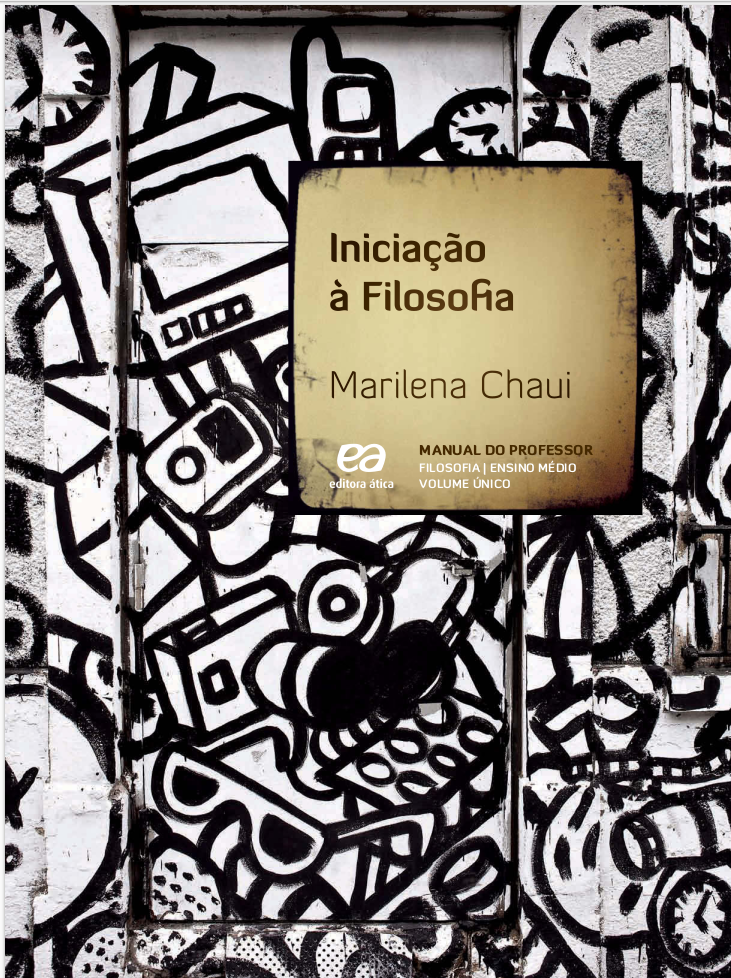
\includegraphics[width=0.5\linewidth]{imagens/Capa-Livro-Introducao-a-Filosofia-MARILENA-CHAUI} 

}

\caption{Livro <b>Introdução à filosofia</b> - CHAUI - 2.ed. - 2013}\label{fig:unnamed-chunk-2}
\end{figure}

\begin{itemize}
\tightlist
\item
  Resumo elaborado para o trabalho de História da Psicologia: ``Mude minha Opinião''.
\item
  Tema do debate: ``O comportamento humano pode ser controlado'';
\end{itemize}

\hypertarget{capuxedtulo-28---a-liberdade}{%
\subsection{Capítulo 28 - A Liberdade}\label{capuxedtulo-28---a-liberdade}}

Esse resumo foi elaborado para apresentação de atividade da disciplina História da Psicologia para segunda nota avaliativa.

\hypertarget{introduuxe7uxe3o}{%
\subsubsection{Introdução}\label{introduuxe7uxe3o}}

\begin{itemize}
\tightlist
\item
  Como é possível SER LIVRE ?

  \begin{itemize}
  \tightlist
  \item
    Se nossa vida transcorre em meio à de outrops indivíduos;
  \item
    Se nossa vida transcorre em meio a instituições sociais;
  \item
    Se nossa vida transcorre em meio a normas culturais;
  \item
    Se nossa vida transcorre em meio às forças da natureza.
  \end{itemize}
\item
  A LIBERDADE é OBJETO CENTRAL dos estudos da ÉTICA como disciplina filosófica;
\item
  A ética dedica-se:

  \begin{itemize}
  \tightlist
  \item
    A DEFINIR e ANALISAR os \textbf{elementos} que (1) \textbf{possibilitam} ou (2) \textbf{impedem} a LIBERDADE;
  \item
    A tratar de duas grandes questões:

    \begin{itemize}
    \tightlist
    \item
      Há limites para a LIBERDADE ?
    \item
      Como e em que termos ela pode ser INTEGRALMENTE CONQUISTADA por todos ?
    \end{itemize}
  \end{itemize}
\end{itemize}

\hypertarget{a-liberdade-como-problema}{%
\subsubsection{A Liberdade como PROBLEMA}\label{a-liberdade-como-problema}}

\begin{itemize}
\tightlist
\item
  Chaiu (2013, p.~278) apresenta duas questões:

  \begin{itemize}
  \tightlist
  \item
    Qual o núcleo da LIBERDADE ?
  \item
    Como podemos sentir a AUSÊNCIA DE LIBERDADE ?
  \end{itemize}
\item
  Ela inicia o diálogo para abordar esses dois problemas apresentando:

  \begin{itemize}
  \tightlist
  \item
    Um POEMA de José Paulo Paes (``O melhor poeta da minha rua'')
  \item
    Um POEMA de Carlos Drummond de Andrade (``Sete faces'')
  \end{itemize}
\item
  Os dois poemas apontam para o grande tema da ética:

  \begin{itemize}
  \tightlist
  \item
    O que está ?
  \item
    O que não está em nosso poder ?
  \item
    Até onde se estende o PODER:

    \begin{itemize}
    \tightlist
    \item
      Da nossa VONTADE ?
    \item
      Do nosso DESEJO ?
    \item
      Da nossa CONSCIÊNCIA ?
    \end{itemize}
  \end{itemize}
\item
  Por fim, até onde se estende o PODER DA NOSSA LIBERDADE ?

  \begin{itemize}
  \tightlist
  \item
    O que ESTÁ EM NOSSO PODER ?
  \item
    O que DEPENDE INTEIRAMENTE DE \textbf{CAUSAS} e \textbf{FORÇAS} EXTERIORES ?
  \end{itemize}
\item
  Mais um poema é apresentado pela autora para consolidar seu raciocínio: Vicente de Carvalho (``Velho tema'')
\item
  Os três poetas nos colocam diante da LIBERDADE como PROBLEMA, seja:

  \begin{itemize}
  \tightlist
  \item
    De modo pessimista (como em José Paulo Paes e Vicente de Carvalho)
  \item
    De modo otimista (como em Carlos Drummond)
  \end{itemize}
\end{itemize}

\hypertarget{a-liberdade-como-questuxe3o-filosuxf3fica}{%
\subsubsection{A Liberdade como QUESTÃO FILOSÓFICA}\label{a-liberdade-como-questuxe3o-filosuxf3fica}}

\begin{itemize}
\tightlist
\item
  A questão da liberdade se apresenta na forma de DOIS PARES OPOSTOS:

  \begin{itemize}
  \tightlist
  \item
    O par necessidade-liberdade

    \begin{itemize}
    \tightlist
    \item
      NECESSIDADE é o termo empregado para se referir ao todo da realidade, existente em si e por si, que age sem nós e nos insere em sua rede de causas e efeitos, condições e consequências.
    \end{itemize}
  \item
    O par contingência-liberdade

    \begin{itemize}
    \tightlist
    \item
      CONTINGÊNCIA ou ACASO significam que a realidade é imprevisível e mutável, impossibilitando deliberação e decisão racionais, definidoras da liberdade.
    \item
      Num mundo onde tudo acontece por acidente, somos como um frágil barquinho perdido num mar tempestuoso, levado em todas as direções, ao sabor das vagas e dos ventos.
    \end{itemize}
  \end{itemize}
\item
  FATALIDADE é o termo usado quando pensamos em forças transcendentes superiores às nossas e que nos governam, quer o queiramos, quer não.
\item
  DETERMINISMO é o termo empregado, a partir do século XIX, para se referir às relações causais necessárias que regem a realidade conhecida e controlada pela ciência;

  \begin{itemize}
  \tightlist
  \item
    No caso da ética, refere-se ao ser humano como objeto das ciências naturais (química e biologia) e das ciências humanas (sociologia e psicologia).
  \item
    Portanto, subordina-o completamente a leis e causas que condicionam seus pensamentos, sentimentos e ações, tornando a liberdade ilusória.
  \end{itemize}
\item
  O que poderia estar em nosso poder?
\item
  Necessidade, fatalidade, determinismo

  \begin{itemize}
  \tightlist
  \item
    Significam que não há lugar para a liberdade, porque o curso das coisas e de nossa vida já está fixado, sem que nele possamos intervir;
  \end{itemize}
\item
  Contingência e acaso

  \begin{itemize}
  \tightlist
  \item
    Significam que não há lugar para a liberdade, porque não há curso algum das coisas e de nossa vida sobre o qual pudéssemos intervir.
  \end{itemize}
\end{itemize}

\hypertarget{truxeas-grandes-concepuxe7uxf5es-filosuxf3ficas-da-liberdade}{%
\subsubsection{Três grandes CONCEPÇÕES FILOSÓFICAS DA LIBERDADE}\label{truxeas-grandes-concepuxe7uxf5es-filosuxf3ficas-da-liberdade}}

\begin{itemize}
\tightlist
\item
  Na mitologia grega NECESSIDADE e CONTINGÊNCIA

  \begin{itemize}
  \tightlist
  \item
    Necessidade: As Moiras ( conhecidas também como Parcas ) eram as três irmãs que determinavam o destino (FATALIDADE), tanto dos deuses, quanto dos seres humanos.
  \item
    A contingência (ou o acaso): Era representada pela Fortuna, mulher volúvel e caprichosa, que trazia nas mãos uma roda, fazendo-a girar de tal modo que quem estivesse no alto (a boa fortuna ou boa sorte) caísse (infortúnio ou má sorte) e quem estivesse embaixo fosse elevado.

    \begin{itemize}
    \tightlist
    \item
      INCONSTANTE, INCERTA e CEGA: a RODA DA FORTUNA era a pura sorte, boa ou má, contra a qual nada se poderia fazer;
    \end{itemize}
  \end{itemize}
\item
  As \textbf{TEORIAS ÉTICAS} procuraram sempre enfrentar o duplo problema da necessidade e da contingência, definindo o campo da liberdade possível
\end{itemize}

\hypertarget{primeira-as-concepuxe7uxf5es-de-aristuxf3teles-e-de-satre}{%
\paragraph{PRIMEIRA: As concepções de Aristóteles e de Satre}\label{primeira-as-concepuxe7uxf5es-de-aristuxf3teles-e-de-satre}}

\begin{itemize}
\tightlist
\item
  ARISTÓTELES

  \begin{itemize}
  \tightlist
  \item
    Postulou a \textbf{PRIMEIRA} grande \textbf{TEORIA FILOSÓFICA DA LIBERDADE} (Livro Ética a Nicômaco)
  \item
    Nesse sentido, a LIBERDADE se opõe ( Necessidade x Contingência )

    \begin{itemize}
    \tightlist
    \item
      Ao que é CONDICIONÁDO EXTERNAMENTE (Necessidade)
    \item
      Ao que ACONTECE SEM ESCOLHA DELIBERADA (Contingência)
    \end{itemize}
  \item
    Afirma que ``É livre aquele que tem em si mesmo o PRINCÍPIO para AGIR ou NÃO AGIR'';
  \item
    LIBERDADE:

    \begin{itemize}
    \tightlist
    \item
      É o poder PLENO e INCONDICIONAL da VONTADE para determinar a si mesmo (\textbf{AUTODETERMINAÇÃO});
    \item
      É uma CAPACIDADE que

      \begin{enumerate}
      \def\labelenumi{\alph{enumi}.}
      \tightlist
      \item
        Não encontra \textbf{obstáculos} para se realizar;
      \item
        Nem é \textbf{forçada} por \textbf{coisa alguma} para agir;
      \end{enumerate}
    \end{itemize}
  \item
    Contingência ( Puro acaso ) x Possível ( Pode acontecer desde que o ser humano DELIBERE e DECIDA realizar uma ação )
  \item
    LIBERDADE:

    \begin{itemize}
    \tightlist
    \item
      É o princípio para escolher entre \textbf{ALTERNATIVAS POSSÍVEIS}
    \item
      Realiza-se:

      \begin{enumerate}
      \def\labelenumi{\alph{enumi}.}
      \tightlist
      \item
        Decisão
      \item
        Ato Voluntário
      \end{enumerate}
    \end{itemize}
  \end{itemize}
\item
  Contrariamente à necessidade e à contingência, sob as quais o agente sofre a ação de uma CAUSA EXTERNA que o OBRIGA A AGIR de determinada maneira no ATO VOLUNTÁRIO LIVRE o agente é causa de si, isto é, CAUSA INTEGRAL DE SUA AÇÃO.
\item
  Sem dúvida, seria possível dizer que a VONTADE LIVRE é determinada:

  \begin{itemize}
  \tightlist
  \item
    Pela RAZÃO;
  \item
    Pela INTELIGÊNCIA;

    \begin{enumerate}
    \def\labelenumi{\alph{enumi}.}
    \tightlist
    \item
      Nesse caso, seria preciso admitir que não é causa de si ou incondicionada
    \item
      Nesse caso é CAUSADA
    \item
      Pelo RACIOCÍNIO;
    \item
      Pelo PENSAMENTO
    \end{enumerate}
  \end{itemize}
\item
  FILÓSOFOS POSTERIORES A ARISTÓTELES

  \begin{itemize}
  \tightlist
  \item
    A INTELIGÊNCIA

    \begin{itemize}
    \tightlist
    \item
      Inclina a VONTADE para certa direção;
    \item
      Não obriga nem constrange a VONTADE
    \item
      Podemos agir na direção contrária à indicada pela inteligência ou razão;
    \end{itemize}
  \end{itemize}
\item
  JEAN-PAUL SATRE

  \begin{itemize}
  \tightlist
  \item
    LIBERDADE

    \begin{itemize}
    \tightlist
    \item
      É a ESCOLHA INCONDICIONAL que o próprio homem faz de seu ser e de seu mundo.
    \item
      Estamos condenados à LIBERDADE;

      \begin{enumerate}
      \def\labelenumi{\alph{enumi}.}
      \tightlist
      \item
        É ela que define a humanidade dos humanos, sem escapatória.
      \end{enumerate}
    \end{itemize}
  \item
    Quando julgamos estar sob o PODER DE FORÇAS EXTERNAS mais poderosas do que nossa VONTADE, esse julgamento é uma decisão livre;

    \begin{itemize}
    \tightlist
    \item
      OUTROS outros homens, nas mesmas circunstâncias, não se curvaram nem se resignaram;
    \end{itemize}
  \item
    QUANDO OUTROS poderiam, nas mesmas circunstâncias, AGIR DE FORMA DIFERENTE a DECISÃO É LIVRE:

    \begin{itemize}
    \tightlist
    \item
      Conformar-se ou resignar-se é uma DECISÃO LIVRE;
    \item
      Afirmar-se ENFRAQUECIDO ou Afirma-se SEM FORÇAS para fazer alguma coisa é uma DECISÃO LIVRE;
    \end{itemize}
  \end{itemize}
\item
  Essa PRIMEIRA concepção \textbf{MANTÉM} a OPOSIÇÃO entre LIBERDADE e NECESSIDADE;
\end{itemize}

\hypertarget{segunda-a-concepuxe7uxe3o-que-une-necessidade-e-liberdade}{%
\paragraph{SEGUNDA: A concepção que une NECESSIDADE e LIBERDADE}\label{segunda-a-concepuxe7uxe3o-que-une-necessidade-e-liberdade}}

\begin{itemize}
\tightlist
\item
  Apresentada:

  \begin{itemize}
  \tightlist
  \item
    Pelo ESTOICISMO no período Helenístico
  \item
    No século XVII com ESPINOSA;
  \item
    No século XIX com HEGEL;
  \end{itemize}
\item
  PRESERVA a ideia ARISTOTÉLICA que:

  \begin{itemize}
  \tightlist
  \item
    A liberdade é AUTODETERMINAÇÃO;
  \item
    É livre quem age sem ser forçado nem constrangido por nada nem por ninguém ( AGIR EXPONTÂNEO )
  \end{itemize}
\item
  DISTANCIA-SE da ideia ARISTOTÉLICA e de SATRE:

  \begin{itemize}
  \tightlist
  \item
    Ao NÃO SITUAR a LIBERDADE no ATO DE ESCOLHA realizado pela VONTADE INDIVIDUAL, \textbf{separada} da NECESSIDADE e OPOSTA A ELA;
  \end{itemize}
\item
  A LIBERDADE é colocada como parte de UM TODO NECESSÁRIO ( AGE LIVREMENTE quem AGE NECESSÁRIAMENTE )
\item
  Para essa perspectiva filosófica, NECESSÁRIO significa aquilo que AGE apenas pela FORÇA INTERNA de sua PRÓPRIA NATUREZA (Estóicos) / SUBSTÂNCIA (Espinosa) / ESPÍRITO (Hegel);
\item
  NATUREZA (Estóicos) / SUBSTÂNCIA (Espinosa) / ESPÍRITO (Hegel) são a TOTALIDADE como PODER ABSOLUTODE AÇÃO;
\item
  Como \textbf{NADA EXTERIOR} obriga a \textbf{NATUREZA}, a \textbf{SUBSTÂNCIA} ou o \textbf{ESPÍRITO} a AGIR, eles são LIVRES, pois agem apenas por seu PODER INTERNO;
\item
  Seu agir é uma NECESSIDADE LIVRE ou uma LIBERDADE NECESSÁRIA porque:

  \begin{itemize}
  \tightlist
  \item
    A NECESSIDADE não é um PODER EXTERNO que obriga a LIBERDADE a AGIR;
  \item
    A NECESSIDADE é apenas a \textbf{LEI INTERNA} que a própria LIBERDADE \textbf{criou para sua própria ação}
  \end{itemize}
\item
  A LIBERDADE não é um PODER INCONDICIONADO PARA ESCOLHER --- a natureza não escolhe, a substância não escolhe, o espírito não escolhe.
\item
  A LIBERDADE é o PODER DO TODO para \textbf{AGIR EM CONFORMIDADE CONSIGO MESMO}:

  \begin{itemize}
  \tightlist
  \item
    Sendo necessariamente O QUE É;
  \item
    Fazendo necessariamente O QUE FAZ;
  \item
    Sendo necessariamente O QUE É;
  \item
    Fazendo necessariamente O QUE FAZ.
  \end{itemize}
\item
  Essa SEGUNDA concepção \textbf{NÃO MANTÉM} a OPOSIÇÃO entre LIBERDADE e NECESSIDADE;

  \begin{itemize}
  \tightlist
  \item
    Ela afirma que a NECESSIDADE é a maneira pela qual a LIBERDADE do TODO se manifesta;
  \item
    A TOTALIDADE

    \begin{itemize}
    \tightlist
    \item
      É LIVRE porque:

      \begin{enumerate}
      \def\labelenumi{\alph{enumi}.}
      \tightlist
      \item
        Se põe a si mesma na existência;
      \item
        Define por si mesma as leis e as regras de sua atividade;
      \end{enumerate}
    \item
      É NECESSÁRIA porque:

      \begin{enumerate}
      \def\labelenumi{\alph{enumi}.}
      \tightlist
      \item
        Tais LEIS e REGRAS exprimem necessariamente \textbf{O QUE ELA É} e \textbf{O QUE ELA FAZ};
      \end{enumerate}
    \end{itemize}
  \end{itemize}
\item
  \textbf{LIBERDADE não é ESCOLHER e DELIBERAR, mas AGIR ou FAZER alguma coisa EM CONFORMIDADE com a NATUREZA DO AGENTE que, no caso, é o TODO}.
\item
  O que é a LIBERDADE HUMANA enquanto o homem é uma parte constituída pelo todo e que age no interior do todo?

  \begin{itemize}
  \tightlist
  \item
    São duas as respostas a essa questão:

    \begin{itemize}
    \tightlist
    \item
      A PRIMEIRA (dada pelos estoicos e por Hegel) afirma que o todo é racional e que suas partes também o são, sendo livres quando agirem em conformidade com as leis racionais do todo, para o bem da totalidade;
    \item
      A SEGUNDA (dada por Espinosa) afirma que as partes são de mesma essência que o todo e, portanto, são RACIONAIS e LIVRES como ele, dotadas de FORÇA INTERIOR para agir por si mesmas, de sorte que a LIBERDADE é TOMAR PARTE ATIVA na atividade do todo.

      \begin{enumerate}
      \def\labelenumi{\alph{enumi}.}
      \tightlist
      \item
        \textbf{TOMAR PARTE ATIVA} significa:
      \item
        Por UM LADO:
        a. Conhecer as CONDIÇÕES e CAUSAS estabelecidas pelo todo;
        b. Conhecer o MODO como elas determinam nossas ações;
      \end{enumerate}

      \begin{itemize}
      \tightlist
      \item
        Por OUTRO LADO (em virtude de tal conhecimento):

        \begin{enumerate}
        \def\labelenumi{\alph{enumi}.}
        \tightlist
        \item
          Não ser um joguete das CONDIÇÕES e CAUSAS que atuam sobre nós
        \item
          AGIR sobre elas também
        \end{enumerate}
      \end{itemize}
    \end{itemize}
  \end{itemize}
\item
  NÃO SOMOS LIVRES para escolher tudo;
\item
  SOMOS LIVRES para fazer tudo quanto esteja de acordo {[} Graças ao conhecimento que temos: (1) de nós mesmos e (2) das circunstâncias {]}:

  \begin{itemize}
  \tightlist
  \item
    Com nosso ser;
  \item
    Com nossa capacidade de agir;
  \end{itemize}
\item
  Para os ESTÓICOS, o homem livre é aquele

  \begin{itemize}
  \tightlist
  \item
    Cuja RAZÃO conhece:

    \begin{itemize}
    \tightlist
    \item
      A necessidade natural;
    \item
      A necessidade de sua própria natureza;
    \end{itemize}
  \item
    Tem força para guiar e dirigir a vontade para que esta exerça um poder absoluto sobre a irracionalidade dos instintos e impulsos, isto é, sobre as paixões.
  \end{itemize}
\item
  Para ESPINOSA, o homem livre é aquele que

  \begin{itemize}
  \tightlist
  \item
    AGE como CAUSA interna, completa e total de sua ação
  \item
    AGE decorrente do \textbf{desenvolvimento espontâneo} da \textbf{essência racional} do agente.
  \item
    Em outras palavras, assim como:

    \begin{itemize}
    \tightlist
    \item
      O todo age livremente pela necessidade de sua essência;
    \item
      O indivíduo livre age por necessidade de sua própria essência.
    \end{itemize}
  \item
    Somos livres quando realizamos nosso ser como uma potência interna capaz de uma pluralidade simultânea de ideias, afetos e ações que decorrem apenas de nosso próprio ser.
  \item
    Somos livres quando:

    \begin{itemize}
    \tightlist
    \item
      O que somos exprimem nossa FORÇA INTERNA para existir e agir
    \item
      O que sentimos exprimem nossa FORÇA INTERNA para existir e agir
    \item
      O que fazemos exprimem nossa FORÇA INTERNA para existir e agir
    \item
      O que pensamos exprimem nossa FORÇA INTERNA para existir e agir.
    \end{itemize}
  \end{itemize}
\item
  Para HEGEL, o homem livre é uma figura que aparece na história e na cultura sob duas formas principais:

  \begin{itemize}
  \tightlist
  \item
    Na primeira, a liberdade humana coincide com o surgimento da cultura

    \begin{itemize}
    \tightlist
    \item
      É livre o homem que não se deixa dominar pela força da natureza e que a vence, dobrando-a à sua vontade

      \begin{enumerate}
      \def\labelenumi{\alph{enumi}.}
      \tightlist
      \item
        Por meio do TRABALHO, da LINGUAGEM e DAS ARTES.
      \item
        Podemos notar que a LIBERDADE refere-se muito mais a uma ATITUDE DA HUMANIDADE, e não do INDIVÍDUO -- a uma vitória da cultura sobre a natureza.
      \end{enumerate}
    \end{itemize}
  \item
    Em sua outra forma, o homem livre como indivíduo livre aparece na história em dois momentos sucessivos:

    \begin{itemize}
    \tightlist
    \item
      O PRIMEIRO é o do surgimento do homem cristão ou o surgimento da interioridade cristã, que descobre a consciência como consciência de si;
    \item
      O SEGUNDO momento, decorrente do primeiro, é o do surgimento da individualidade racional moderna ou do indivíduo como consciência de si reflexiva
    \item
      Nesse momento, o indivíduo vê SUA RAZÃO e SUA VONTADE:

      \begin{enumerate}
      \def\labelenumi{\alph{enumi}.}
      \tightlist
      \item
        Independentes da natureza ou da necessidade natural;
      \item
        Independentes da coação de autoridades externas \textbf{na definição de seu pensamento e de sua vontade}.
      \end{enumerate}
    \end{itemize}
  \end{itemize}
\end{itemize}

\hypertarget{terceira-a-concepuxe7uxe3o-da-liberdade-como-possibilidade-objetiva}{%
\paragraph{TERCEIRA: A concepção da liberdade como POSSIBILIDADE OBJETIVA}\label{terceira-a-concepuxe7uxe3o-da-liberdade-como-possibilidade-objetiva}}

\begin{itemize}
\tightlist
\item
  Essa terceira concepção busca \textbf{UNIR ELEMENTOS DAS DUAS OUTRAS};
\item
  Essa terceira concepção afirma:

  \begin{itemize}
  \tightlist
  \item
    COMO NA SEGUNDA: Que não somos um poder incondicional de escolha entre quaisquer possíveis, mas que nossas escolhas são condicionadas pelas circunstâncias em que vivemos:

    \begin{itemize}
    \tightlist
    \item
      Naturais;
    \item
      Psíquicas;
    \item
      Culturais; e
    \item
      Históricas.
    \end{itemize}
  \end{itemize}
\item
  COMO NA PRIMEIRA: Que a liberdade é um ato de DECISÃO e ESCOLHA entre vários possíveis.

  \begin{itemize}
  \tightlist
  \item
    Todavia, não se trata da liberdade de querer alguma coisa, e sim (como já dizia Espinosa) de fazer alguma coisa;
  \item
    Somos livres para fazer alguma coisa quando temos o poder de fazê-la.
  \end{itemize}
\item
  Essa TERCEIRA concepção da liberdade:

  \begin{itemize}
  \tightlist
  \item
    Encontramos:

    \begin{itemize}
    \tightlist
    \item
      Em pensadores marxistas (como Georg Lukács e Lucien Goldmann);
    \item
      Em pensadores vindos da fenomenologia;
    \item
      Em pensadores vindos do existencialismo (como Merleau-Ponty)
    \end{itemize}
  \item
    Introduz a NOÇÃO DE POSSIBILIDADE OBJETIVA

    \begin{itemize}
    \tightlist
    \item
      O possível não é apenas alguma coisa sentida ou percebida subjetivamente por nós
    \item
      O possível é também, e sobretudo, alguma coisa inscrita objetivamente no seio da própria necessidade

      \begin{enumerate}
      \def\labelenumi{\alph{enumi}.}
      \tightlist
      \item
        Que indica que o curso de uma situação pode ser mudado por nós, em certas direções e sob certas condições.
      \end{enumerate}
    \end{itemize}
  \item
    A LIBERDADE:

    \begin{itemize}
    \tightlist
    \item
      É a capacidade para perceber tais possibilidades
    \item
      É o poder para realizar aquelas ações que mudam o curso das coisas, dando-lhe outra direção ou outro sentido.
    \end{itemize}
  \end{itemize}
\item
  De fato:

  \begin{itemize}
  \tightlist
  \item
    EXISTIRAM FILÓSOFOS que afirmaram a LIBERDADE COMO UM PODER ABSOLUTAMENTE INCONDICIONAL DA VONTADE (como o fizeram, por razões diferentes,Kant e Sartre);
  \item
    EXISTIRAM OUTROS FILÓSOFOS que levaram em conta a TENSÃO entre nossa LIBERDADE e as CONDIÇÕES -- naturais, culturais, psíquicas -- que nos determinam.
  \end{itemize}
\item
  As discussões

  \begin{itemize}
  \tightlist
  \item
    Sobre

    \begin{itemize}
    \tightlist
    \item
      as paixões
    \item
      os interesses
    \item
      as circunstâncias histórico-sociais;
    \item
      as condições naturais;
    \end{itemize}
  \item
    Sempre estiveram presentes na ética
  \item
    Por isso, uma ideia como a de possibilidade objetiva sempre esteve pressuposta ou implícita nas TEORIAS SOBRE LIBERDADE.
  \end{itemize}
\end{itemize}

\hypertarget{a-morte-e-a-vida}{%
\paragraph{A morte e a Vida}\label{a-morte-e-a-vida}}

\begin{itemize}
\tightlist
\item
  Viver e morrer são a descoberta da finitude humana, de nossa temporalidade e de nossa identidade;
\item
  A MORTE, e somente ela, completa o que somos, dizendo o que fomos;
\item
  Por isso, os filósofos estoicos propunham que

  \begin{itemize}
  \tightlist
  \item
    Somente após a morte, quando terminam as vicissitudes da vida, podemos afirmar que alguém foi feliz ou infeliz.
  \item
    ``Quem não souber morrer bem terá vivido mal'', afirmou o estoico Sêneca
  \end{itemize}
\item
  Enquanto vivos, somos tempo e mudança, estamos sendo;
\item
  Os filósofos existencialistas disseram:

  \begin{itemize}
  \tightlist
  \item
    A existência precede a essência
  \item
    Nossa essência é a síntese do todo de nossa existência.
  \end{itemize}
\item
  Morrer é um ato solitário. Morre-se só: a essência da morte é a solidão.
\item
  A ética

  \begin{itemize}
  \tightlist
  \item
    É o mundo das relações intersubjetivas,isto é, entre o eu e o outro como sujeitos e pessoas
  \item
    É o eu e o outro como seres

    \begin{itemize}
    \tightlist
    \item
      Conscientes;
    \item
      Livres; e
    \item
      Responsáveis.
    \end{itemize}
  \end{itemize}
\item
  Nenhuma experiência evidencia tanto a dimensão essencialmente intersubjetiva da vida e da vida ética quanto a do DIÁLOGO.
\item
  Porque a vida é intersubjetividade corporal e psíquica e porque a vida ética é reciprocidade entre sujeitos;
\item
  Espinosa afirma que

  \begin{itemize}
  \tightlist
  \item
    O ser humano é mais livre na companhia dos outros do que na solidão;
  \item
    ``somente os seres humanos livres são gratos e reconhecidos uns aos outros'', pois os sujeitos livres são aqueles que ``nunca agem com fraude, mas sempre de boa-fé''.
  \end{itemize}
\end{itemize}

\hypertarget{p1---leitura-e-produuxe7uxe3o-textual}{%
\chapter{P1 - Leitura e Produção Textual}\label{p1---leitura-e-produuxe7uxe3o-textual}}

Neste capítulo estarão contidos os resumos capítulos de livros, artigos, monografias, dissertações, teses relacionados com a disciplina Leitura e Produção Textual.

\hypertarget{artigo-a-importuxe2ncia-de-um-sistema-de-sauxfade-puxfablico-e-universal-no-enfrentamento-uxe0-epidemia}{%
\section{\texorpdfstring{Artigo: \href{https://www.epsjv.fiocruz.br/noticias/reportagem/a-importancia-de-um-sistema-de-saude-publico-e-universal-no-enfrentamento-a}{A importância de um sistema de saúde público e universal no enfrentamento à epidemia}}{Artigo: A importância de um sistema de saúde público e universal no enfrentamento à epidemia}}\label{artigo-a-importuxe2ncia-de-um-sistema-de-sauxfade-puxfablico-e-universal-no-enfrentamento-uxe0-epidemia}}

\hypertarget{referuxeancia-bibliogruxe1fica}{%
\subsection{Referência Bibliográfica}\label{referuxeancia-bibliogruxe1fica}}

\hypertarget{resumo}{%
\subsection{Resumo}\label{resumo}}

\hypertarget{resenha}{%
\subsection{Resenha}\label{resenha}}

\hypertarget{artigo-psicologia-da-sauxfade-contexto-e-intervenuxe7uxe3o-da-revista-anuxe1lise-psicoluxf3gica}{%
\section{\texorpdfstring{Artigo: \href{https://drive.google.com/file/d/1Xph9Bpk8TS42f-cGZP08vVJ3TLEqK3GZ/view?usp=sharing}{Psicologia da Saúde: Contexto e intervenção}** da Revista \textbf{Análise Psicológica}''}{Artigo: Psicologia da Saúde: Contexto e intervenção** da Revista Análise Psicológica''}}\label{artigo-psicologia-da-sauxfade-contexto-e-intervenuxe7uxe3o-da-revista-anuxe1lise-psicoluxf3gica}}

\hypertarget{referuxeancia-bibliografica}{%
\subsection{Referência Bibliografica}\label{referuxeancia-bibliografica}}

CARVALHO TEIXEIRA, José A.; LEAL, Isabel. Psicologia da Saúde: Contexto e intervenção. Revista Análise Psicológica, v. 4, n.~VIII, p.~453-458, 1990.

\hypertarget{resumo-1}{%
\subsection{Resumo}\label{resumo-1}}

\begin{enumerate}
\def\labelenumi{\arabic{enumi}.}
\tightlist
\item
  \textbf{Introdução}
\end{enumerate}

\begin{itemize}
\tightlist
\item
  A Expressão Psicologia da Saúde

  \begin{itemize}
  \tightlist
  \item
    Foi definida por Matarazzo (1980)
  \item
    CONCEITO: É a área disciplinar que diz respeito ao «papel da Psicologia como CIÊNCIA e como PROFISSÃO nos domínios da saúde e das medicinas comportamentais»
  \end{itemize}
\item
  O CONCEITO de PSICOLOGIA DA SAÚDE unificou e tomou como referências dois campos interdisciplinares

  \begin{itemize}
  \tightlist
  \item
    SAÚDE COMPORTAMENTAL

    \begin{itemize}
    \tightlist
    \item
      Se refere essencialmente à DIMENSÃO PREVENTIVA
    \item
      Uma subespecialidade interdisciplinar que se ocupa especificamente:

      \begin{itemize}
      \tightlist
      \item
        Da promoção da saúde;
      \item
        Da prevenção da doença;
      \item
        De disfunções em pessoas habitualmente saudáveis;
      \end{itemize}
    \end{itemize}
  \item
    MEDICINA COMPORTAMENTAL

    \begin{itemize}
    \tightlist
    \item
      Remete para as DIMENSÕES CURATIVA e de REABILITAÇÃO;
    \item
      Aproxima mais a Psicologia com as diversas especialidades médicas e cirúrgicas;
    \item
      Um campo interdisciplinar de prática clínica e de investigação que diz respeito a doença e a disfunções psicológicas com ela relacionadas.
    \end{itemize}
  \item
    CONCEITO DOS AUTORES: PSICOLOGIA DA SAÚDE

    \begin{itemize}
    \tightlist
    \item
      É a intervenção psicológica no campo da saúde e que melhor parece corresponder as necessidades da prática clínica.
    \item
      Permite integrar harmoniosamente os TRÊS NÍVEIS clássicos de PREVENÇÃO: primária, secundária e terciária
    \end{itemize}
  \end{itemize}
\item
  A abordagem psicológica da saúde e da doença é uma resposta a necessidade de humanização dos cuidados de saúde;
\item
  A Psicologia da Saúde é uma resposta a (1) necessidade essencial de INTERDISCIPLINARIEDADE da investigação científica e (2) a necessidade de uma COMUNICAÇÃO EFETIVA ( que alcance os RESULTADOS PRETENDIDOS )
\item
  O discurso médico e o discurso psicológico em Psicologia da Saúde.
\item
  Como será possível o diálogo interdisciplinar em Psicologia da Saúde ?
\item
  O que espera-se da Psicologia em Psicologia da Saúde ?

  \begin{itemize}
  \tightlist
  \item
    Que a Psicologia se mantenha e assegure:

    \begin{itemize}
    \tightlist
    \item
      Sua identidade própria; e
    \item
      Sua autonomia.
    \end{itemize}
  \end{itemize}
\end{itemize}

\begin{enumerate}
\def\labelenumi{\arabic{enumi}.}
\setcounter{enumi}{1}
\tightlist
\item
  \textbf{Contexto}
\end{enumerate}

\begin{itemize}
\tightlist
\item
  Psicologia da Saúde como \textbf{movimento mútuo de aproximação} entre a Psicologia e a Medicina
\item
  Década de 70: O modelo clássico \textbf{BIOMÉDICO} e a proposta do modelo \textbf{BIOPSICOSOCIAL} de Engel(1970) e Lipowski(1977)

  \begin{itemize}
  \tightlist
  \item
    \textbf{Consequências} do novo \textbf{modelo BIOPSICOSSOCIAL}:

    \begin{itemize}
    \tightlist
    \item
      Foco na \textbf{PESSOA DOENTE} ao invés de na \textbf{DOENÇA}
    \item
      Compreensão mais ampliada \textbf{do ADOECER} e \textbf{do ESTAR DOENTE} correlacionando com:

      \begin{itemize}
      \tightlist
      \item
        Condutas individuais;
      \item
        Personalidade;
      \item
        Estilo relacional;
      \item
        Outros aspectos psicológicos;
      \item
        Outros aspectos psicossociais.
      \end{itemize}
    \end{itemize}
  \end{itemize}
\item
  \textbf{Estilos individuais} de lidar com a \textbf{ADVERSIDADE}
\item
  Os \textbf{modelos psicológicos}: Pespectivas COMPORTAMENTAL, PSICANALÍTICA e SISTEMÁTICA

  \begin{itemize}
  \tightlist
  \item
    Perspectiva COMPORTAMENTAL;
  \item
    Perspectiva PSICANALÍTICA;
  \item
    Perspectiva SISTEMÁTICA.
  \end{itemize}
\item
  A progressiva \textbf{NECESSIDADE} de relacionar a Psicologia com a saúde física

  \begin{itemize}
  \tightlist
  \item
    Decorrente do duplo enraizamento do MODELO BIOPSICOSSOCIAL e dos MODELOS PSICOLÓGICOS (perspectivas COMPORTAMENTAL, PSICANALÍTICA e SISTEMÁTICA)
  \item
    Provocando o repensar da formação médica e da formação psicológica
  \end{itemize}
\item
  \textbf{Áreas de interesse} da Psicologia da Saúde (Subespecialidade da Psicologia Clínica)

  \begin{itemize}
  \tightlist
  \item
    Estudo da ADAPTAÇÃO PSICOLÓGICA e ALTERAÇÕES DO COMPORTAMENTO associadas:

    \begin{itemize}
    \tightlist
    \item
      Ao envelhecimento;
    \item
      À deterioração neurológica;
    \item
      À maternidade;
    \item
      Às doenças crônicas.
    \end{itemize}
  \item
    Investigação do \textbf{PAPEL} e da \textbf{INFLUÊNCIA} de fatores PSICOLÓGICOS e da PERSONALIDADE:

    \begin{itemize}
    \tightlist
    \item
      CAUSALIDADE MULTIFATORIAL:

      \begin{itemize}
      \tightlist
      \item
        De doenças corporais;
      \item
        Na EVOLUÇÃO, TRATAMENTO e REABILITAÇÃO de doenças corporais;
      \end{itemize}
    \end{itemize}
  \item
    Influência de VARIAVEIS PSICOLÓGICAS em ÁREAS PSICOLÓGICAS

    \begin{itemize}
    \tightlist
    \item
      Respostas individuais a vários tratamentos médicos
    \item
      Estudo de Compliance
    \item
      As RESPOSTAS PSICOLÓGICAS aos PROCEDIMENTOS CIRÚRGICOS
    \item
      O IMPACTO PSICOLÓGICO da HOSPITALIZAÇÃO
    \item
      O tratamento da DOR CRÔNICA
    \item
      Aspectos interativos do stress
    \item
      coping e adaptação
    \item
      Doenças terminais
    \end{itemize}
  \item
    Abordagem psicológica de PROMOÇÃO DA SAÚDE

    \begin{itemize}
    \tightlist
    \item
      Determinantes das mudanças de ESTILOS DE VIDA relacionados com a saúde;
    \end{itemize}
  \item
    Estudo dos ASPECTOS PSICOLÓGICOS associados ao

    \begin{itemize}
    \tightlist
    \item
      Stress, Tabagismo, Obesidade,Diabetes, Doenças cardiovasculares, Asma Brônquica e Doenças cancerosas;
    \item
      Necessidade de Avaliação;
    \item
      Necessidade de Aoio Apsicológico;
    \item
      Problemas decorrentes de novas tecnologias
    \item
      Tecnologia de Transplantes;
    \item
      Tecnologias de Reprodução;
    \end{itemize}
  \end{itemize}
\item
  O que é PSICOLOGIA DA SAÚDE

  \begin{itemize}
  \tightlist
  \item
    É um PROCESSO em constante mudança (DEVIR) que tende para superação das perspectivas reducionistas da Medicina ( Através de MODELOS INTEGRATIVOS da SAÚDE e da DOENÇA );
  \item
    É uma SUBESPECIALIDADE da PSICICOLOGIA CLÍNICA

    \begin{itemize}
    \tightlist
    \item
      Psicologia (Como CIÊNCIA e como PROFISSÃO)
    \item
      Onde a Psicologia:

      \begin{itemize}
      \tightlist
      \item
        Atua ativamente no campo da saúde e da doença;
      \item
        Dialoga produtivamente com a Medicina ( Mantendo seus MODELOS, DISCURSO e AUTONOMIA )
      \end{itemize}
    \item
      Onde as REALIDADES PSICOLÓGICAS tornam-se mais relevantes

      \begin{itemize}
      \tightlist
      \item
        Na PROMOÇÃO DA SAÚDE;
      \item
        Na PREVENÇÃO DA DOENÇA;
      \item
        No Adoecer;
      \item
        No Estar-doente
      \item
        Na recuperação;
      \item
        Na reabilitação conducente à reinserção familiar e comunitária
      \end{itemize}
    \end{itemize}
  \item
    CAMPOS DE INTERESSE da PSICOLOGIA DA SAÚDE

    \begin{itemize}
    \tightlist
    \item
      Estudo dos COMPORTAMENTOS DE RISCO para SAÚDE;
    \item
      Estudo dos COMPORTAMENTOS NECESSÁRIOS para MANUTENÇÃO DA SAÚDE;
    \item
      Cognições relacionadas com a saúde e com a doença;
    \item
      Aspectos psicológicos da adesão aos tratamentos;
    \item
      Aspectos psicológicos dos ambientes dos serviços de saúde;
    \item
      Estratégias de COPING relacionadas com a DOENÇA e com a INCAPACIDADE;
    \item
      Relações entre cuidados com a saúde e a qualidade de vida
    \item
      Aquisição precoce de COMPORTAMENTOS para a saúde;
    \item
      As condições de saúde dos técnicos de saúde;
    \end{itemize}
  \item
    ATIVIDADES da PSICOLOGIA DA SAÚDE ( Por possuir DISCURSO PRÓPRIO e AUTONOMIA )

    \begin{itemize}
    \tightlist
    \item
      Prevenção de saúde;
    \item
      Avaliação de saúde;
    \item
      Apoio Psicológico ligado aos cuidados de saúde;
    \item
      Investigações ligadas aos cuidados de saúde;
    \end{itemize}
  \end{itemize}
\item
  Dada a COMPLEXIDADE DE QUESTÕES que a Psicologia tem que tratar, existe DIVERSIDADE:

  \begin{itemize}
  \tightlist
  \item
    De modelos de formação;
  \item
    De modelos de informação;
  \item
    De contribuições teóricas
  \item
    De modelos de intervençaõ;
  \end{itemize}
\item
  COMO TRABALHA o PSICÓLOGO CLÍNICO com Psicologia da Saúde:

  \begin{itemize}
  \tightlist
  \item
    APLICANDO

    \begin{itemize}
    \tightlist
    \item
      Teorias básicas
    \item
      Metodologias de avaliação
    \item
      Metodologias de investigação
    \item
      Modelos de intervenção da Psicologia no campo da saúde
    \end{itemize}
  \item
    Numa PERSPECTIVA DE ABORDAGEM: Globalizante
  \end{itemize}
\item
  Funcionamento BIOLÓGICO x funcionamento PSICOLÓGICO (Roessler \& Decker, 1986).

  \begin{itemize}
  \tightlist
  \item
    DISFUNÇÕES BIOLÓGICAS podem produzir reações adversas ao FUNCIONAMENTO PSICOLÓGICO
  \item
    MUDANÇAS PSICOLÓGICAS e SOCIAIS podem produzir alterações no FUNCIONAMENTO BIOLÓGICO;
  \end{itemize}
\end{itemize}

\begin{enumerate}
\def\labelenumi{\arabic{enumi}.}
\setcounter{enumi}{2}
\tightlist
\item
  \textbf{Intervenção}
\end{enumerate}

\begin{itemize}
\tightlist
\item
  O OBJETO da Psicologia da Saúde ( definição ainda IMPRECISA )

  \begin{itemize}
  \tightlist
  \item
    É a EXPERIÊNCIA PSICOLÓGICA
  \item
    É a RELAÇÃO que os sujeitos estabelecem:

    \begin{itemize}
    \tightlist
    \item
      Com seu estado de saúde ou de doença;
    \item
      Com acontecimentos que associam-se frequentemente a MOMENTOS DE CRISE:

      \begin{itemize}
      \tightlist
      \item
        Gravidez;
      \item
        Puberdade;
      \item
        Envelhecimento;
      \item
        Menopausa;
      \end{itemize}
    \item
      Com especificidades biológicas
    \end{itemize}
  \end{itemize}
\item
  A PSICOLOGIA DA SAÚDE trabalha com vivências que o sujeito

  \begin{itemize}
  \tightlist
  \item
    Experimenta
  \item
    Projeta
  \item
    Reativa
  \end{itemize}
\item
  Para PSICOLOGIA DA SAÚDE o que INTERESSA são:

  \begin{itemize}
  \tightlist
  \item
    As FORMAS pelas quais o sujeito lida com os acontecimentos
  \item
    Os MOTIVOS pelos quais o sujeito lida com os acontecimentos
  \end{itemize}
\item
  O CONCEITO DE SAÚDE

  \begin{itemize}
  \tightlist
  \item
    Bem-estar físico, psicológico e social:

    \begin{itemize}
    \tightlist
    \item
      Do sujeito
    \item
      Do grupo
    \item
      Da comunidade
    \end{itemize}
  \item
    É mais que a AUSÊNCIA DE SINTOMAS
  \item
    É mais que DESVIOS em relação à MÉDIA
  \item
    É um sentir-se bem INDIVIDUALIZADO e SUBJETIVO
  \item
    TRADUZ uma representação social da nossa época
  \item
    É centrada no HOMEM e não na patologia ou entidades nosológicas;
  \end{itemize}
\item
  Os OBJETIVOS e METODOLOGIAS da Psicologia da Saúde

  \begin{itemize}
  \tightlist
  \item
    São os objetivos específicos da Psicologia Geral
  \item
    São os específicos da Psicologias Clínica
  \item
    São centrados sobre um terreno que recebe da Medicina as suas CATEGORIAS DE INTERVENÇÃO
  \end{itemize}
\item
  OS OBJETIVOS da PSICOLOGIA DA SAÚDE são: ( O que a Psicologia da Saúde pretende ? Em resumo, que o sujeito possa lidar o melhor possível com a nova situação )

  \begin{itemize}
  \tightlist
  \item
    Optimização dos RECURSOS AFETIVOS e COGNITIVOS do sujeito
  \item
    Adoção de ESTRATÉGIAS adequadas para SUPERAÇÃO DE CRISES
  \item
    REFORÇO de DEFESAS eventualmente enfraquecidas
  \end{itemize}
\item
  Exemplos de Atividades de INTERVENÇÃO em Psicologia da Saúde

  \begin{itemize}
  \tightlist
  \item
    Prevenção, avaliação, tratamento e reabilitação de disfunções psicológicas em doentes físicos;
  \item
    Aconselhamento e troca de informações com os outros técnicos de saúde sobre aspectos psicológicos (e psicossociais) dedoentes físicos, particularmente em estudos de casos individuais;
  \item
    Tratamento psicológico de reacções psicológicas as doenças físicas, com incidência particular na experiência vivida da doença e das suas limitações;
  \item
    Prevenção e/ou tratamento de condutas desajustadas que são consequência ou mesmo parte integrante das doenças corporais;
  \item
    Identificação e suporte de sujeitos em risco psicológico colocados perante o adoecer corporal;
  \item
    Aconselhamento e suporte de problemas familiares relacionados com a doença física de um dos seus membros;
  \item
    Facilitação da comunicação entre as pessoas doentes e as equipas de saúde, prevenindo conflitos potenciais e manejando os manifestos;
  \item
    Participação activa em programas de reabilitação de doentes físicos, particularmente com doenças crónicas invalidantes e exigindo processo activo de reabilitação psicológica e psicossocial;
  \item
    Investigação nas áreas de intervenção dos factores psicológicos nas doenças corporais e, ainda, na organização e funcionamento dos serviços de saúde e seu impacto psicológico sobre as pessoas doentes;
  \item
    Estudo e implementação da modificação de comportamentos e de estilos de vida, necessária para a conservação da saúde e prevenção da doença.\\
  \end{itemize}
\item
  Modelo psicológicos de INFORMAÇÃO, FORMAÇÃO e INTERVENÇÃO em Psicologia da Saúde

  \begin{itemize}
  \tightlist
  \item
    Não existe um modelo único, existem vários;
  \item
    Usam-se vários modelos de acordo com as NECESSIDADES e CIRCUNSTÂNICAS de cada caso individual, sempre com a necessária FLEXIBILIDADE indispensável a prática clínica;
  \end{itemize}
\item
  Os INSTRUMENTOS FUNDAMENTAIS de INTERVENÇÃO ( Específicos da Clínica Psicológica )

  \begin{itemize}
  \tightlist
  \item
    Entrevista clínica
  \item
    Exame Psicológico
  \item
    Psicoterapia
  \end{itemize}
\item
  A importância da PSICOTERAPIA em Psicologia da Saúde

  \begin{itemize}
  \tightlist
  \item
    O que habitualmente se pede ao Psicólogo Clínico:

    \begin{itemize}
    \tightlist
    \item
      Que colabore na CLARIFICAÇÃO de uma situação
    \item
      Que ajude o sujeito a MUDAR, PROMOVENDO um melhor ajustamento psicológico:

      \begin{itemize}
      \tightlist
      \item
        À situação
      \item
        Às consequências da situação
      \end{itemize}
    \end{itemize}
  \end{itemize}
\item
  Definição de PSICOTERAPIA DE APOIO

  \begin{itemize}
  \tightlist
  \item
    Uma forma de tratamento psicológico para sujeitos com problemas físicos (ou mentais crónicos) para os quais a MUDANÇA RADICAL não
    constitui um OBJETIVO REALISTA (Sidney Bloch,1979).
  \item
    Ela não inviabiliza:

    \begin{itemize}
    \tightlist
    \item
      Outra alternativa psocoterapêutica ulterior;
    \item
      Qualquer encaminhamento considerado adequado ou possível
    \end{itemize}
  \item
    Os OBJETIVOS da PSICOTERAPIA DE APOIO

    \begin{itemize}
    \tightlist
    \item
      Promover o melhor funcionamento psicológico possível, reforçando as capacidades do sujeito para lidar com os vários aspectos da sua vida e com a adversidade;
    \item
      Aumentar a auto-estima e tornar a pessoa cada vez mais consciente da realidade;
    \item
      Prevenir as eventuais recidivas, combater a dependência e outros factores que possam contribuir para o aparecimento de cronicidade psicológica;
    \item
      Vir a transferir a fonte de apoio (pelo menos em parte) para a família e rede social de apoio.
    \end{itemize}
  \end{itemize}
\item
  Os COMPONENTES PRINCIPAIS da INTERVENÇÃO terapêutica

  \begin{itemize}
  \tightlist
  \item
    Transmissão de segurança;
  \item
    Explicação;
  \item
    Sugestão;
  \item
    Aconselhamento;
  \item
    Encorajamento;
  \item
    Modificação de circunstâncias ambienciais;
  \item
    Permissão para a exteriorização emocional e afectiva
  \item
    Uso de técnicas de intervenção cognitiva e comportamental diversas, consoante as especificidades do sujeito e da situação que podem ser ÚTEIS EM SITUAÇÕES ESPECÍFICAS:

    \begin{itemize}
    \tightlist
    \item
      Tratamento da dor crónica;
    \item
      Mudança de comportamentos de risco em doentes coronários;
    \item
      Preparação psicológica para a cirurgia;
    \item
      Tabagismo, etc.
    \end{itemize}
  \end{itemize}
\item
  A Psicologia da Saúde é um reencontro entre a CONGIÇÃO e o AFETO.
\item
  \textbf{OBSERVAÇÃO}:

  \begin{itemize}
  \tightlist
  \item
    Definição de COPING: ``tentativa ou empenho para lidar com exigências externas (do ambiente) ou internas (do próprio sujeito) percebidas como sobrecarregando ou excedendo os recursos da pessoa.''(Folkman e Lazarus)'' \href{https://www.psicologia.pt/artigos/ver_opiniao.php?codigo=AOP0216}{Site \textbf{Psicologia.pt}}
  \end{itemize}
\end{itemize}

\hypertarget{resenha-1}{%
\subsection{Resenha}\label{resenha-1}}

\hypertarget{p1---metodologia-cientuxedfica}{%
\chapter{P1 - Metodologia Científica}\label{p1---metodologia-cientuxedfica}}

capa-livro-fundamentos-metodologia-cientifica-lakatos.png

\hypertarget{resumo-do-livro-fundamentos-de-metodologia-cientuxedfica-marconi-lakatos-teixeira-2017}{%
\section{\texorpdfstring{Resumo do Livro ``\textbf{Fundamentos de Metodologia Científica}'' (MARCONI; LAKATOS; TEIXEIRA, 2017)}{Resumo do Livro ``Fundamentos de Metodologia Científica'' (MARCONI; LAKATOS; TEIXEIRA, 2017)}}\label{resumo-do-livro-fundamentos-de-metodologia-cientuxedfica-marconi-lakatos-teixeira-2017}}

Figura - Livro ``Fundamentos de Metodologia Científica'' (MARCONI; LAKATOS; TEIXEIRA, 2017)

\hypertarget{capuxedtulo-8---pesquisa}{%
\subsection{Capítulo 8 - Pesquisa}\label{capuxedtulo-8---pesquisa}}

\hypertarget{conceito-de-pesquisa}{%
\subsubsection{Conceito de Pesquisa}\label{conceito-de-pesquisa}}

\begin{itemize}
\tightlist
\item
  \textbf{Bagno} (2010, p.~17 apud MARCONI; LAKATOS, p.~185) afirma que a palavra PESQUISA chegou até o Português através do Espanhol, que por sua vez assimilou do Latim:

  \begin{itemize}
  \tightlist
  \item
    Latim \emph{PERQUIRO}:

    \begin{itemize}
    \tightlist
    \item
      \textbf{Significado}: 1. Procurar por toda parte; buscar com cuidado. 2.Inquirir. 3. Perguntar; indagar bem, aprofundar na busca
    \item
      O significado dessa palavra em Latim insiste na \textbf{ideia de uma busca feita com cuidado e profundidade}.
    \end{itemize}
  \end{itemize}
\item
  \textbf{Ander-Egg} (1978, p.~28 apud MARCONI; LAKATOS, p.~185) a PESQUISA é:

  \begin{itemize}
  \tightlist
  \item
    Um PROCEDIMENTO:

    \begin{itemize}
    \tightlist
    \item
      Formal
    \item
      Reflexivo ( Método de Pensamento );
    \item
      Sistemático;
    \item
      Controlado;
    \item
      Crítico
    \end{itemize}
  \item
    Que PERMITE, em qualquer campo do conhecimento, DESCOBRIR

    \begin{itemize}
    \tightlist
    \item
      Novos fatos ou dados;
    \item
      Relações ou leis
    \end{itemize}
  \item
    Que REQUER

    \begin{itemize}
    \tightlist
    \item
      Tratamento científico
    \end{itemize}
  \item
    Que CONSTITUI

    \begin{itemize}
    \tightlist
    \item
      Caminho para CONHECER A REALIDADE
    \item
      Caminho para CONHECER VERDADES PARCIAIS
    \end{itemize}
  \end{itemize}
\end{itemize}

\hypertarget{passos-para-desenvolvimento-de-um-projeto-de-pesquisa}{%
\subsubsection{Passos para DESENVOLVIMENTO DE UM PROJETO DE PESQUISA}\label{passos-para-desenvolvimento-de-um-projeto-de-pesquisa}}

\begin{enumerate}
\def\labelenumi{\arabic{enumi}.}
\tightlist
\item
  \textbf{Seleção} do tópico (Problema) para investigação;
\item
  \textbf{Definição} e \textbf{diferenciação} do problema;
\item
  \textbf{Levantamento} de hipóteses de trabalho;
\item
  \textbf{Coleta}, \textbf{sistematização} e \textbf{classificação} dos dados;
\item
  \textbf{Análise} e \textbf{interpretação} dos dados;
\item
  \textbf{Elaboração} do relatório do resultado da pesquisa
\end{enumerate}

\hypertarget{planejamento-da-pesquisa}{%
\paragraph{Planejamento da Pesquisa}\label{planejamento-da-pesquisa}}

\hypertarget{preparauxe7uxe3o-da-pesquisa}{%
\paragraph{Preparação da Pesquisa}\label{preparauxe7uxe3o-da-pesquisa}}

\begin{enumerate}
\def\labelenumi{\arabic{enumi}.}
\tightlist
\item
  Decisão;
\item
  Especificação dos objetivos;
\item
  Elaboração de um plano de trabalho;
\item
  Constituição da equipe de trabalho;
\item
  Levantamento de recursos e cronograma
\end{enumerate}

\hypertarget{fases-da-pesquisa}{%
\subsubsection{Fases da Pesquisa}\label{fases-da-pesquisa}}

\begin{enumerate}
\def\labelenumi{\arabic{enumi}.}
\tightlist
\item
  Escolha do tema;
\item
  Levantamento de dados;
\item
  Formulação do problema;
\item
  Definição dos termos;
\item
  Construção de hipóteses;
\item
  Indicação de variáveis;
\item
  Delimitação da pesquisa;
\item
  Amostragem;
\item
  Seleção de métodos e técnicas;
\item
  Organização do instrumental de pesquisa;
\item
  Teste de instrumentos e procedimentos
\end{enumerate}

\hypertarget{execuuxe7uxe3o-da-pesquisa}{%
\subsubsection{Execução da Pesquisa}\label{execuuxe7uxe3o-da-pesquisa}}

\begin{enumerate}
\def\labelenumi{\arabic{enumi}.}
\tightlist
\item
  C3oleta de dados;
\item
  Elaboração dos dados;
\item
  Análise e interpretação dos dados;
\item
  Representação dos dados;
\item
  Conclusões
\end{enumerate}

\hypertarget{relatuxf3rio-de-pesquisa}{%
\subsubsection{Relatório de Pesquisa}\label{relatuxf3rio-de-pesquisa}}

\hypertarget{planejamento-da-pesquisa-preparauxe7uxe3o-da-pesquisa}{%
\subsubsection{PLANEJAMENTO DA PESQUISA: Preparação da Pesquisa}\label{planejamento-da-pesquisa-preparauxe7uxe3o-da-pesquisa}}

\hypertarget{decisuxe3o}{%
\paragraph{Decisão}\label{decisuxe3o}}

\begin{itemize}
\tightlist
\item
  Esse é o momento em que o pesquisador \textbf{toma a decisão} de \textbf{realizar ou não realizar} a pesquisa;
\item
  A pesquisa pode ser realizada \textbf{no INTERESSE}:

  \begin{itemize}
  \tightlist
  \item
    Do Próprio Pesquisador;
  \item
    De Alguém
  \item
    De Alguma Entidade;
  \end{itemize}
\item
  Nem sempre é fácil se dereminar \textbf{o que se pretente investigar}
\item
  A INVESTIGAÇÃO PRESSUPÕE:

  \begin{itemize}
  \tightlist
  \item
    Uma série de CONHECIMENTOS ANTERIORES;
  \item
    Metodologia adequada
  \end{itemize}
\end{itemize}

\hypertarget{especificauxe7uxe3o-dos-objetivos}{%
\paragraph{Especificação dos objetivos}\label{especificauxe7uxe3o-dos-objetivos}}

\begin{itemize}
\tightlist
\item
  O OBJETIVO torna \textbf{EXPLÍCITO O PROBLEMA};
\item
  Os OBJETIVOS orientam a pesquisa para se \textbf{SABER}:

  \begin{itemize}
  \tightlist
  \item
    O QUE se vai PROCURAR;
  \item
    O QUE se pretende ALCANÇAR
  \end{itemize}
\item
  Os objetivos devem \textbf{SER}

  \begin{itemize}
  \tightlist
  \item
    LIMITADOS
  \item
    CLARAMENTE DEFINIDOS
  \end{itemize}
\item
  Os objetivos podem \textbf{DEFINIR}

  \begin{itemize}
  \tightlist
  \item
    A natureza do trabalho;
  \item
    O tipo do problema;
  \item
    O material a coletar
  \end{itemize}
\end{itemize}

\begin{Shaded}
\begin{Highlighting}[]
\NormalTok{flowchart LR}
\NormalTok{A(Os \textless{}b\textgreater{}OBJETIVOS\textless{}/b\textgreater{}){-}{-}\textgreater{}B(Podem SER)}
\NormalTok{A{-}{-}\textgreater{}C(Respondem as PERGUNTAS)}
\NormalTok{C{-}{-}\textgreater{}R(Por Quê?)}
\NormalTok{C{-}{-}\textgreater{}S(Para Quê)}
\NormalTok{C{-}{-}\textgreater{}T(Para Quem?)}
\NormalTok{B{-}{-}\textgreater{}D((a))}
\NormalTok{D{-}{-}\textgreater{}H(Intrínsecos)}
\NormalTok{D{-}{-}\textgreater{}M(Extrínsecos)}
\NormalTok{B{-}{-}\textgreater{}E((b))}
\NormalTok{E{-}{-}\textgreater{}I(Teóricos)}
\NormalTok{E{-}{-}\textgreater{}N(Práticos)}
\NormalTok{B{-}{-}\textgreater{}F((c))}
\NormalTok{F{-}{-}\textgreater{}J(Gerais)}
\NormalTok{F{-}{-}\textgreater{}O(Específicos)}
\NormalTok{B{-}{-}\textgreater{}G((d))}
\NormalTok{G{-}{-}\textgreater{}K(De CURTO Prazo)}
\NormalTok{G{-}{-}\textgreater{}P(De LONGO Prazo)}
\end{Highlighting}
\end{Shaded}

\hypertarget{elaborauxe7uxe3o-de-um-plano-de-trabalho}{%
\paragraph{Elaboração de um plano de trabalho}\label{elaborauxe7uxe3o-de-um-plano-de-trabalho}}

\begin{itemize}
\tightlist
\item
  É um passo a passo de como o trabalho de pesquisa será realizado que facilita ou aumenta as suas chances de viabilidade;
\item
  Imprime ordem lógica a sua execução;
\item
  Tornam claros os RECURSOS \textbf{materiais}, \textbf{humanos} e de \textbf{tempo} necessários a sua execução;
\item
  \textbf{Pode} ou \textbf{não} ser alterado durante sua execução;
\end{itemize}

\hypertarget{constituiuxe7uxe3o-da-equipe-de-trabalho}{%
\paragraph{Constituição da equipe de trabalho}\label{constituiuxe7uxe3o-da-equipe-de-trabalho}}

\begin{itemize}
\tightlist
\item
  Engloba

  \begin{itemize}
  \tightlist
  \item
    Recrutamento de pessoal;
  \item
    Treinamento de pessoal;
  \item
    Distribuição de tarefas;
  \item
    Indicação dos locais de trabalho;
  \item
    Indicação dos materiais e equipamentos
  \end{itemize}
\item
  \textbf{Observação}: A pesquisa também pode ser realizada por \textbf{uma pessoa} apenas.
\end{itemize}

\hypertarget{levantamento-de-recursos-e-cronograma}{%
\paragraph{Levantamento de recursos e cronograma}\label{levantamento-de-recursos-e-cronograma}}

\begin{itemize}
\tightlist
\item
  O pesquisados deve fazer DE ANTEMÃO a previsão dos gastos necessários para a realização da pesquisa ( orçamento o mais aproximado possível do montante de recursos );
\item
  Não pode falta um cronograma para executar a pesquisa em cada uma de suas etapas
\end{itemize}

\begin{Shaded}
\begin{Highlighting}[]
\NormalTok{flowchart LR}
\NormalTok{A(O \textless{}b\textgreater{}CRONOGRAMA\textless{}/b\textgreater{} e\textless{}br\textgreater{}Os \textless{}b\textgreater{}RECURSOS\textless{}/b\textgreater{}){-}{-}\textgreater{}C(Respondem as PERGUNTAS)}
\NormalTok{C{-}{-}\textgreater{}R(Quando ?)}
\NormalTok{C{-}{-}\textgreater{}S(Quanto ?)}
\end{Highlighting}
\end{Shaded}

\hypertarget{planejamento-da-pesquisa-fases-da-pesquisa}{%
\subsubsection{PLANEJAMENTO DA PESQUISA: Fases da Pesquisa}\label{planejamento-da-pesquisa-fases-da-pesquisa}}

\hypertarget{escolha-do-tema}{%
\paragraph{Escolha do tema;}\label{escolha-do-tema}}

\begin{itemize}
\tightlist
\item
  O \textbf{TEMA} é o \textbf{ASSUNTO} que se deseja estudar e pesquisar;
\item
  A \textbf{DEFINIÇÃO DO TEMA} pode perdurar por toda a pesquisa e deverá ser \textbf{FREQUENTEMENTE REVISTO};
\item
  ESCOLHA um TEMA/ASSUNTO

  \begin{itemize}
  \tightlist
  \item
    Que MEREÇA ser investigado cientificamente;
  \item
    Que TENHA CONDIÇÕES de ser, em função da pesquisa:

    \begin{itemize}
    \tightlist
    \item
      Formulado;
    \item
      Delimitado
    \item
      Exequível (disponibilidade de tempo do pesquisador, background acadêmico, recursos, etc\ldots)
    \end{itemize}
  \end{itemize}
\item
  O TEMA/ASSUNTO deve SER:

  \begin{itemize}
  \tightlist
  \item
    Preciso
  \item
    Bem determinado
  \item
    Específico
  \end{itemize}
\end{itemize}

\begin{Shaded}
\begin{Highlighting}[]
\NormalTok{flowchart LR}
\NormalTok{A(A \textless{}b\textgreater{}escolha do TEMA\textless{}/b\textgreater{}){-}{-}\textgreater{}B(Responde a PERGUNTA){-}{-}\textgreater{}C(\textless{}b\textgreater{}O QUE\textless{}/b\textgreater{} será\textless{}br\textgreater{}PESQUISADO/EXPLORADO ?)}
\end{Highlighting}
\end{Shaded}

\hypertarget{levantamento-de-dados}{%
\paragraph{Levantamento de dados;}\label{levantamento-de-dados}}

\begin{itemize}
\tightlist
\item
  São TRÊS as formas de OBTENÇÃO DE DADOS:

  \begin{itemize}
  \tightlist
  \item
    Pesquisa Bibliográfica
  \item
    Pesquisa Documental
  \item
    Contatos Diretos
    \#\#\#\#\# Pesquisa Bibliográfica
  \end{itemize}
\item
  Apanhado geral sobre os \textbf{principais trabalhos realizados}
\item
  Procura-se, relacionados ao TEMA:

  \begin{itemize}
  \tightlist
  \item
    Dados atuais;
  \item
    Dados relevantes;
  \item
    Indícios importantes
  \item
    Subsídios importantes
  \end{itemize}
\item
  Pode orientar indagações sore a pesquisa
\item
  ANTES de qualquer PESQUISA DE CAMPO deve-se realizar uma ANÁLISE MINUCIOSA de FONTES DOCUMENTAIS que sirvam de suporte à pesquisa
\end{itemize}

\hypertarget{investigauxe7uxe3o-preliminar}{%
\paragraph{Investigação Preliminar}\label{investigauxe7uxe3o-preliminar}}

\begin{itemize}
\tightlist
\item
  Também chamada de \textbf{ESTUDO EXPLORATÓRIO}.
\item
  Deve ser realizada através de \textbf{DOIS ASPECTOS}:

  \begin{itemize}
  \tightlist
  \item
    \textbf{DOCUMENTOS}

    \begin{itemize}
    \tightlist
    \item
      \textbf{PRINCIPAIS TIPOS DE DOCUMENTOS}

      \begin{enumerate}
      \def\labelenumi{\alph{enumi}.}
      \tightlist
      \item
        Fontes \textbf{PRIMÁRIAS}:
      \item
        Dados Históricos;
      \item
        Dados Bibliográficos;
      \item
        Dados Estatísticos;
      \item
        Documentação \textbf{pessoal};
        a. Autobiografias
        b. Certidão de nascimento
        c.~Certidão de óbito
        d.~Diários
        e. Memórias
      \item
        Registros de natureza pública/privada
      \item
        Fontes \textbf{SECUNDÁRIOS}
      \item
        Imprensa em geral
      \item
        Obras literárias
      \end{enumerate}
    \end{itemize}
  \item
    \textbf{CONTATOS DIRETOS / PESQUISA DE CAMPO / PESQUISA DE LABORATÓRIO}

    \begin{itemize}
    \tightlist
    \item
      São realizados com PESSOAS que podem \textbf{fornecer os dados diretamente};
    \item
      São realizadas com PESSOAS que podem \textbf{sugerir fontes de informações úteis};
    \end{itemize}
  \end{itemize}
\end{itemize}

\hypertarget{formulauxe7uxe3o-do-problema}{%
\paragraph{Formulação do problema;}\label{formulauxe7uxe3o-do-problema}}

\begin{itemize}
\tightlist
\item
  PROBLEMA:

  \begin{itemize}
  \tightlist
  \item
    É uma DIFICULDADE, teórica ou prática, NO CONHECIMENTO de alguma coisa;
  \item
    É uma DIFICULDADE para a qual SE QUER ENCONTRAR uma solução;
  \end{itemize}
\end{itemize}

\hypertarget{definiuxe7uxe3o-do-problema}{%
\paragraph{Definição do Problema}\label{definiuxe7uxe3o-do-problema}}

\begin{itemize}
\tightlist
\item
  O que é \textbf{DEFINIR O PROBLEMA} ?

  \begin{itemize}
  \tightlist
  \item
    É especificar a \textbf{DIFICULDADE} em detalhes precisos e exatos;
  \item
    É especificar a \textbf{DIFICULDADE} com clareza, concisão e objetividade
  \end{itemize}
\item
  A \textbf{CLAREZA DO PROBLEMA} ajuda na CONTRUÇÃO DA HIPÓTESE CENTRAL;
\item
  \textbf{COMO DEVE SER DEFINIDO} o \textbf{PROBLEMA} ?

  \begin{itemize}
  \tightlist
  \item
    Na forma INTERROGATIVA
  \item
    Delimitando-o de forma a indicar as \textbf{VARIÁVEIS} que \textbf{AFETAM O ESTUDO} com possíveis \textbf{RELAÇÕES ENTRE SI}.
  \end{itemize}
\item
  A \textbf{FORMULAÇÃO DE UM PROBLEMA}

  \begin{itemize}
  \tightlist
  \item
    Requer \textbf{CONHECIMENTOS PRÉVIOS} no assunto, exigindo:

    \begin{itemize}
    \tightlist
    \item
      Materiais informativos
    \item
      Imaginação criadora
    \end{itemize}
  \end{itemize}
\item
  Deve-se evitar PROBLEMAS MUITO ABRANGENTES, pois tornam a pesquisa MAIS COMPLEXA;
\end{itemize}

\hypertarget{apuxf3s-a-definiuxe7uxe3o-do-problema}{%
\paragraph{APÓS a Definição do Problema}\label{apuxf3s-a-definiuxe7uxe3o-do-problema}}

\begin{itemize}
\tightlist
\item
  \textbf{APÓS FORMULADO UM PROBLEMA}, segue-se as \textbf{ETAPAS VALORATIVAS}, analisando-se:

  \begin{itemize}
  \tightlist
  \item
    \textbf{Viabilidade}: pode ser eficazmente resolvido através da pesquisa?
  \item
    \textbf{Relevância}: é capaz de trazer conhecimentos novos?
  \item
    \textbf{Novidade}: está adequado ao estádio atual da evolução científica?
  \item
    \textbf{Exequibilidade}: om esse problema, é possível chegar a uma conclusão
    válida?
  \item
    \textbf{Oportunidade}: o problema atende a INTERESSES \textbf{particulares} e \textbf{gerais}?
  \end{itemize}
\end{itemize}

\hypertarget{forma-de-conceber-um-problema-cientuxedfico}{%
\paragraph{Forma de conceber um problema científico}\label{forma-de-conceber-um-problema-cientuxedfico}}

\begin{itemize}
\tightlist
\item
  Qual o OBJETIVO DO TRABALHO DE PESQUISA ?

  \begin{itemize}
  \tightlist
  \item
    PROBLEMA de : estudo descritivo, de caráter informativO explicativo ou preditivo;
  \item
    PROBLEMA de \textbf{INFORMAÇÃO}: coleta de dados a respeito de estruturas e condutas observáveis, dentro de uma área de fenômenos;
  \item
    PROBLEMA de de \textbf{AÇÃO}: campos de ação onde determinados conhecimento
    sejam aplicados com êxito.
  \item
    INVESTIGAÇÃO \textbf{PURA} e \textbf{APLICADA}: estuda um problema relativo ao conhecimento científico ou à sua aplicabilidade.
  \end{itemize}
\end{itemize}

\begin{Shaded}
\begin{Highlighting}[]
\NormalTok{flowchart LR}
\NormalTok{A(A \textless{}b\textgreater{}Formulação do\textless{}br\textgreater{}PROBLEMA\textless{}/b\textgreater{}){-}{-}\textgreater{}B(Responde as PERGUNTAS){-}{-}\textgreater{}C(\textless{}b\textgreater{}O QUÊ\textless{}/b\textgreater{}?)}
\NormalTok{B{-}{-}\textgreater{}D(\textless{}b\textgreater{}COMO ?\textless{}/b\textgreater{})}
\end{Highlighting}
\end{Shaded}

\hypertarget{definiuxe7uxe3o-dos-termos}{%
\paragraph{Definição dos termos;}\label{definiuxe7uxe3o-dos-termos}}

\begin{itemize}
\tightlist
\item
  É tornar os TERMOS DA PESQUISA claros, compreensivos, objetivos e adequados que possam dar margem a interpretações errôneas;
\item
  O uso de termos apropriados, consistentemente definidos, CONTRIBUI para a \textbf{melhor compreensão da REALIDADE OBSERVADA};
\item
  Há TERMOS que precisam ser compreendidos com um \textbf{SIGNIFICADO ESPECÍFICO};
\item
  Há dois \textbf{TIPOS DE DEFINIÇÕES}:

  \begin{itemize}
  \tightlist
  \item
    \textbf{SIMPLES}: apenas traduzem o significado do termo ou expressão meno
    conhecida;
  \item
    \textbf{OPERACIONAL}: além do significado, ajudam, com exemplos, na
    compreensão do conceito, tornando clara a experiência no mundo
    extensional.
  \end{itemize}
\end{itemize}

\hypertarget{construuxe7uxe3o-de-hipuxf3teses}{%
\paragraph{Construção de hipóteses;}\label{construuxe7uxe3o-de-hipuxf3teses}}

\hypertarget{indicauxe7uxe3o-de-variuxe1veis}{%
\paragraph{Indicação de variáveis;}\label{indicauxe7uxe3o-de-variuxe1veis}}

\hypertarget{delimitauxe7uxe3o-da-pesquisa}{%
\paragraph{Delimitação da pesquisa;}\label{delimitauxe7uxe3o-da-pesquisa}}

\hypertarget{amostragem}{%
\paragraph{Amostragem;}\label{amostragem}}

\hypertarget{seleuxe7uxe3o-de-muxe9todos-e-tuxe9cnicas}{%
\paragraph{Seleção de métodos e técnicas;}\label{seleuxe7uxe3o-de-muxe9todos-e-tuxe9cnicas}}

\hypertarget{organizauxe7uxe3o-do-instrumental-de-pesquisa}{%
\paragraph{Organização do instrumental de pesquisa;}\label{organizauxe7uxe3o-do-instrumental-de-pesquisa}}

\hypertarget{teste-de-instrumentos-e-procedimentos}{%
\subsubsection{Teste de instrumentos e procedimentos}\label{teste-de-instrumentos-e-procedimentos}}

\begin{itemize}
\tightlist
\item
\end{itemize}

  \bibliography{referencias.bib,packages.bib}

\end{document}
